% !TeX encoding = UTF-8
% !TeX spellcheck = es_ES
\documentclass{article}
\usepackage{fullpage}
\usepackage[utf8]{inputenc}
\usepackage{pict2e}
\usepackage{amsmath}
\usepackage{enumitem}
\usepackage{eurosym}
\usepackage{mathtools}
\usepackage{amssymb, amsfonts, latexsym, cancel}
\usepackage{graphicx}
\usepackage{fontenc}
\usepackage{setspace}
\usepackage{adjustbox}
\usepackage{float}
\setstretch{1.35}
\renewcommand{\arraystretch}{1.3}
\setlength\columnsep{20pt}
\usepackage{bold-extra}
\usepackage{subcaption}
\graphicspath{ {images/} }
\usepackage{tcolorbox}
\usepackage{xcolor, colortbl}
\usepackage{wrapfig}
\usepackage{empheq}
\usepackage{array}
\usepackage{parskip}
\usepackage{arydshln}
\renewcommand*\contentsname{\color{black}Índice} 
\usepackage{array, multirow, multicol}
\definecolor{lightblue}{HTML}{007AFF}
\usepackage{color}
\usepackage{etoolbox}
\usepackage{listings}
\usepackage{mdframed}
\setlength{\parindent}{0pt}
\usepackage{underscore}
\usepackage{hyperref}
\usepackage{tikz}
\usetikzlibrary{shapes, positioning, patterns}
\usepackage{tikz-qtree}
\usepackage{biblatex}
\usepackage{pdfpages}
\usepackage{pgfplots}
\usepackage{pgfkeys}
\usepackage{mathrsfs}
\addbibresource{biblatex-examples.bib}
\usepackage[a4paper, left=1cm, right=1.5cm, top=1cm,
bottom=1.5cm]{geometry}
\everymath{\displaystyle}
\usetikzlibrary{decorations.pathreplacing, calc}
\usepackage{titlesec}
\usepackage{pgffor}
\usepackage{subcaption}
\usepackage{venndiagram}
\setlength{\fboxrule}{1.5pt}

% Configura el formato de las secciones utilizando titlesec
\titleformat{\section}
{\color{red}\normalfont\LARGE\bfseries}
{Tema \thesection:}
{10 pt}
{}

\titleformat{\subsection}
{\normalfont\Large\bfseries\color{red}}{\thesubsection)}{1em}{\color{lightblue}}

\titleformat{\subsubsection}
{\normalfont\large\bfseries\color{red}}{\thesubsubsection)}{1em}{\color{lightblue}}

\newcommand{\bboxed}[1]{\fcolorbox{lightblue}{lightblue!10}{$#1$}}
\newcommand{\rboxed}[1]{\fcolorbox{red}{red!10}{$#1$}}

\newcommand{\bu}[1]{\textcolor{lightblue}{\underline{#1}}}
\newcommand{\lb}[1]{\textcolor{lightblue}{#1}}
\newcommand{\db}[1]{\textcolor{blue}{#1}}
\newcommand{\rc}[1]{\textcolor{red}{#1}}

\newcommand{\dx}{\:\mathrm{d}x}
\newcommand{\dt}{\:\mathrm{d}t}
\newcommand{\dy}{\:\mathrm{d}y}
\newcommand{\dz}{\:\mathrm{d}z}
\newcommand{\dth}{\:\mathrm{d}\theta}
\newcommand{\dr}{\:\mathrm{d}\rho}
\newcommand{\du}{\:\mathrm{d}u}
\newcommand{\dv}{\:\mathrm{d}v}
\newcommand{\tozero}[1]{\cancelto{0}{#1}~~~}
\newcommand{\lbb}[2]{\textcolor{lightblue}{\underbracket[1pt]{\textcolor{black}{#1}}_{#2}}}
\newcommand{\dbb}[2]{\textcolor{blue}{\underbracket[1pt]{\textcolor{black}{#1}}_{#2}}}
\DeclareMathOperator{\N}{\mathbb{N}}
\DeclareMathOperator{\Z}{\mathbb{Z}}
\DeclareMathOperator{\R}{\mathbb{R}}
\DeclareMathOperator{\Q}{\mathbb{Q}}
\DeclareMathOperator{\K}{\mathbb{K}}
\DeclareMathOperator{\lcm}{lcm}

\renewcommand{\mod}{~\mathrm{mod}~}

\newcommand{\rbinom}[2]{\dfrac{#1!}{#2!\cdot(#1-#2)!}}

\renewcommand{\CancelColor}{\color{lightblue}}

\begin{document}
\section{Lógica}

\begin{enumerate}[label=\color{red}\textbf{\arabic*)}, leftmargin=*]
      \item \lb{Consideremos las proposiciones $p$ \textit{me gusta comer} y $q$ \textit{me gusta beber}. Proporcionar una expresión coloquial sencilla para las proposiciones $\neg p,\: p\vee q, \:p\wedge q, \:p\vee\neg q,\neg p\wedge q$.}
      \begin{itemize}[label=\color{red}$\to$]
            \item $\db{\neg p:}$ No me gusta comer
            \item $\db{p\vee q:}$ Me gusta comer o beber
            \item $\db{p\wedge q:}$ Me gusta comer y beber
            \item $\db{p\vee \neg q:}$ Me gusta comer y no beber
            \item $\db{\neg p\wedge q:}$ Me gusta beber y no comer
      \end{itemize}
      \item \lb{Encontrar la tabla de verdad de $\neg p\wedge q$.}
      
      $\begin{array}{|c|c|c|c|}
            \hline
            \lb{p} & \lb{q} & \lb{\neg p} & \lb{\neg p\wedge q} \\ \hline
            1 & 1 & 0 & 0 \\
            1 & 0 & 0 & 0 \\
            0 & 1 & 1 & 1 \\
            0 & 0 & 1 & 0 \\ \hline 
      \end{array}$
      \item \lb{Encontrar la tabla de verdad de las siguientes proposiciones:}
      \begin{enumerate}[label=\color{red}\alph*)]
            \item $\db{(p\wedge q)\to p}$
            
            $\begin{array}{|c|c|c|c|}
            \hline
            \lb{p} & \lb{q} & \lb{p\wedge q} & \lb{(p\wedge q)\to p} \\  \hline
            1 & 1 & 1 & 1 \\ 
            1 & 0 & 0 & 1 \\ 
            0 & 1 & 0 & 1 \\ 
            0 & 0 & 0 & 1\\ \hline
            \end{array} $
            \item $\db{(p\vee q)\to q}$
            
            $\begin{array}{|c|c|c|c|}
            \hline
            \lb{p} & \lb{q} & \lb{p\vee q} & \lb{(p\vee q)\to q} \\  \hline
            1 & 1 & 1 & 1 \\ 
            1 & 0 & 1 & 0 \\ 
            0 & 1 & 1 & 1 \\ 
            0 & 0 & 0 & 1 \\ \hline
            \end{array} $
            \item $\db{p\to(q\vee r)}$
            
            $\begin{array}{|c|c|c|c|c|}
            \hline
            \lb{p} & \lb{q} & \lb{r} & \lb{q\vee r} & \lb{p\to(q\vee r)} \\  \hline
            1 & 1 & 1 & 1 & 1 \\ 
            1 & 1 & 0 & 1 & 1 \\ 
            1 & 0 & 1 & 1 & 1 \\ 
            1 & 0 & 0 & 0 & 0 \\ 
            0 & 1 & 1 & 1 & 1 \\ 
            0 & 1 & 0 & 1 & 1 \\ 
            0 & 0 & 1 & 1 & 1 \\ 
            0 & 0 & 0 & 0 & 1 \\ \hline
            \end{array} $
            \item $\db{p\leftrightarrow(p\vee q)\leftrightarrow q}$
            
            $\begin{array}{|c|c|c|c|c|}
            \hline
            \lb{p} & \lb{q} & \lb{p\vee q} & \lb{p\leftrightarrow (p\vee q)} & \lb{p\leftrightarrow(p\vee q)\leftrightarrow q} \\  \hline
            1 & 1 & 1 & 1 & 1 \\ 
            1 & 0 & 1 & 1 & 0 \\ 
            0 & 1 & 1 & 0 & 0 \\ 
            0 & 0 & 0 & 1 & 0 \\ \hline
            \end{array} $
            \item $\db{(p\vee q\wedge r)\to\neg p\vee q}$
            
            $\begin{array}{|c|c|c|c|c|c|c|c|}
                  \hline
                  \lb{p} & \lb{q} & \lb{r} & \lb{\neg p} & \lb{q \wedge r} & \lb{p\vee q\wedge r} & \lb{(p\vee q\wedge r)\to\neg p} & \lb{(p\vee q\wedge r)\to\neg p\vee q} \\ \hline
                  1 & 1 & 1 & 0 & 1 & 1 & 0 & 1 \\
                  1 & 1 & 0 & 0 & 0 & 1 & 0 & 1 \\
                  1 & 0 & 1 & 0 & 0 & 1 & 0 & 0 \\
                  1 & 0 & 0 & 0 & 0 & 1 & 0 & 0 \\
                  0 & 1 & 1 & 1 & 1 & 1 & 1 & 1 \\
                  0 & 1 & 0 & 1 & 0 & 0 & 1 & 1 \\
                  0 & 0 & 1 & 1 & 0 & 0 & 1 & 1 \\
                  0 & 0 & 0 & 1 & 0 & 0 & 1 & 1 \\ \hline
            \end{array}$
            \item $\db{\neg(\neg p\to\neg q\vee r)}$ 
            
            $\begin{array}{|c|c|c|c|c|c|c|c|}
                  \hline
                  \lb{p} & \lb{q} & \lb{r} & \lb{\neg p} & \lb{\neg q} & \lb{\neg q\vee r} & \lb{\neg p\to\neg q\vee r} & \lb{\neg(\neg p\to\neg q\vee r)} \\ \hline
                  1 & 1 & 1 & 0 & 0 & 1 & 1 & 0 \\
                  1 & 1 & 0 & 0 & 0 & 0 & 1 & 0 \\
                  1 & 0 & 1 & 0 & 1 & 1 & 1 & 0 \\
                  1 & 0 & 0 & 0 & 1 & 1 & 1 & 0 \\
                  0 & 1 & 1 & 1 & 0 & 1 & 1 & 0 \\
                  0 & 1 & 0 & 1 & 0 & 0 & 0 & 1 \\
                  0 & 0 & 1 & 1 & 1 & 1 & 1 & 0 \\
                  0 & 0 & 0 & 1 & 1 & 1 & 1 & 0 \\ \hline
            \end{array}$
      \end{enumerate}
      \item \lb{Comprobar que $p\vee \neg(p\wedge q)$ es una tautología}
      
      $\begin{array}{|c|c|c|c|c|}
            \hline
            \lb{p} & \lb{q} & \lb{p\wedge q} & \lb{\neg (p\wedge q)} & \lb{p\vee \neg(p\wedge q)} \\ \hline
            1 & 1 & 1 & 0 & 1 \\
            1 & 0 & 0 & 1 & 1 \\
            0 & 1 & 0 & 1 & 1 \\
            0 & 0 & 0 & 1 & 1 \\ \hline
      \end{array}$
      
      Es una tautología.
      \item \lb{Demostrar que las proposiciones $\neg(p\wedge q)$ y $\neg p\vee \neg q$ son lógicamente equivalentes.}
      
      Según las leyes de DeMorgan $\neg(p\wedge q)$ y $\neg p\vee \neg q$ son lógicamente equivalentes. Ahora se puede comprobar con las tablas de verdad:
      
      $\begin{array}{|c|c|c|c||c|c||c|}
            \hline
            \lb{p} & \lb{q} & \lb{\neg p} & \lb{\neg q} & \lb{p\wedge q} & \lb{\neg(p\wedge q)} & \lb{\neg p\vee \neg q} \\ \hline
            1 & 1 & 0 & 0 & 1 & 0 & 0 \\
            1 & 0 & 0 & 1 & 0 & 1 & 1 \\
            0 & 1 & 1 & 0 & 0 & 1 & 1 \\
            0 & 0 & 1 & 1 & 0 & 1 & 1 \\ \hline
      \end{array}$
      Queda demostrado.
      \item \lb{Dada la proposición $p\to q$, ¿existirá alguna de entre la siguiente lista que sea lógicamente equivalente? La lista es $q\to p,\neg p\to\neg q$ y $\neg q\to \neg p$ que se denomina recíproca, inversa y contrapositiva, respectivamente.}
      
      Dada la proposición condicional $p\to q$, su contrapositiva es equivalente ya que una es verdadera sí, y sólo si lo es la otra.
      \item \lb{¿Cuáles de las siguientes proposiciones son equivalentes?}
      \begin{enumerate}[label=\color{red}\alph*)]
            \item \db{$\neg(p\wedge q)$ y $\neg p\vee q$.}
            
            $\begin{array}{|c|c|c||c|c||c|}
                  \hline
                  \lb{p} & \lb{q} & \lb{\neg p} & \lb{p\wedge q} & \lb{\neg(p\wedge q)} & \lb{\neg p\vee q} \\ \hline
                  1 & 1 & 0 & 1 & 0 & 1 \\
                  1 & 0 & 0 & 0 & 1 & 0 \\
                  0 & 1 & 1 & 0 & 1 & 1 \\
                  0 & 0 & 1 & 0 & 1 & 1 \\ \hline
            \end{array}$
            
            No son equivalentes
            \item \db{$p\to(\neg q)$ y $\neg p\vee\neg q$.}
            
            $\begin{array}{|c|c|c|c||c||c|}
                  \hline
                  \lb{p} & \lb{q} & \lb{\neg p} & \lb{\neg q} & \lb{p\to(\neg q)} & \lb{\neg p\vee \neg q} \\ \hline
                  1 & 1 & 0 & 0 & 0 & 0 \\
                  1 & 0 & 0 & 1 & 1 & 1 \\
                  0 & 1 & 1 & 0 & 1 & 1 \\
                  0 & 0 & 1 & 1 & 1 & 1 \\ \hline
            \end{array}$
            
            Son equivalentes.
            \item \db{$p\wedge q\vee r\wedge q$ y $(p\wedge r)\vee q$.}
            
            $\begin{array}{|c|c|c||c|c|c||c|c|}
                  \hline
                  \lb{p} & \lb{q} & \lb{r} & \lb{p\wedge q} & \lb{r\wedge q} & \lb{p\wedge q\vee r\wedge q} & \lb{p\wedge r} & \lb{(p\wedge r)\vee q} \\ \hline
                  1 & 1 & 1 & 1 & 1 & 1 & 1 & 1 \\
                  1 & 1 & 0 & 1 & 0 & 1 & 0 & 1 \\
                  1 & 0 & 1 & 0 & 0 & 0 & 1 & 1 \\
                  1 & 0 & 0 & 0 & 0 & 0 & 0 & 0 \\
                  0 & 1 & 1 & 0 & 1 & 1 & 0 & 1 \\
                  0 & 1 & 0 & 0 & 0 & 0 & 0 & 1 \\
                  0 & 0 & 1 & 0 & 0 & 0 & 0 & 0 \\
                  0 & 0 & 0 & 0 & 0 & 0 & 0 & 0 \\ \hline
            \end{array}$
            
            No son equivalentes
            \item \db{$p\vee q\wedge r\vee q$ y $(p\vee r)\wedge q$.}
            
            $\begin{array}{|c|c|c||c|c|c||c|c|}
                  \hline
                  \lb{p} & \lb{q} & \lb{r} & \lb{p\wedge q} & \lb{r\wedge q} & \lb{p\wedge q\vee r\wedge q} & \lb{p\vee r} & \lb{(p\vee r)\wedge q} \\ \hline
                  1 & 1 & 1 & 1 & 1 & 1 & 1 & 1 \\
                  1 & 1 & 0 & 1 & 0 & 1 & 1 & 1 \\
                  1 & 0 & 1 & 0 & 0 & 0 & 1 & 0 \\
                  1 & 0 & 0 & 0 & 0 & 0 & 1 & 0 \\
                  0 & 1 & 1 & 0 & 1 & 1 & 1 & 1 \\
                  0 & 1 & 0 & 0 & 0 & 0 & 0 & 0 \\
                  0 & 0 & 1 & 0 & 0 & 0 & 1 & 0 \\
                  0 & 0 & 0 & 0 & 0 & 0 & 0 & 0 \\ \hline
            \end{array}$
            
            Son equivalentes 
            \item \db{$p\leftrightarrow (q\leftrightarrow r)$ y $(p\leftrightarrow q)\leftrightarrow r$.}
            
            $\begin{array}{|c|c|c||c|c||c|c|}
                  \hline
                  \lb{p} & \lb{q} & \lb{r} & \lb{q\leftrightarrow r} & \lb{p\leftrightarrow(q\leftrightarrow r)} & \lb{p\leftrightarrow q} & \lb{(p\leftrightarrow q)\leftrightarrow r} \\ \hline
                  1 & 1 & 1 & 1 & 1 & 1 & 1 \\
                  1 & 1 & 0 & 0 & 0 & 1 & 0 \\
                  1 & 0 & 1 & 0 & 0 & 0 & 0 \\
                  1 & 0 & 0 & 1 & 1 & 0 & 1 \\
                  0 & 1 & 1 & 1 & 0 & 0 & 0 \\
                  0 & 1 & 0 & 0 & 1 & 0 & 1 \\
                  0 & 0 & 1 & 0 & 1 & 1 & 1 \\
                  0 & 0 & 0 & 1 & 0 & 1 & 0 \\ \hline
            \end{array}$
            
            Son equivalentes
            \item \db{$p\to(q\to r)$ y $(p\to q)\to r$.}
            
            $\begin{array}{|c|c|c||c|c||c|c|}
                  \hline
                  \lb{p} & \lb{q} & \lb{r} & \lb{q\to r} & \lb{p\to(q\to r)} & \lb{p\to q} & \lb{(p\to q)\to r} \\ \hline
                  1 & 1 & 1 & 1 & 1 & 1 & 1 \\
                  1 & 1 & 0 & 0 & 0 & 1 & 0 \\
                  1 & 0 & 1 & 1 & 1 & 0 & 1 \\
                  1 & 0 & 0 & 1 & 1 & 0 & 1 \\
                  0 & 1 & 1 & 1 & 1 & 1 & 1 \\
                  0 & 1 & 0 & 0 & 1 & 1 & 0 \\
                  0 & 0 & 1 & 1 & 1 & 1 & 1 \\
                  0 & 0 & 0 & 1 & 1 & 1 & 0 \\ \hline
            \end{array}$
            
            No son equivalentes
      \end{enumerate}
      \item \lb{Escribir la negación de las siguientes proposiciones de la forma más sencilla posible.}
      \begin{enumerate}[label=\color{red}\alph*)]
            \item \db{Si ella trabaja, ganará dinero.}
            
            Si ella no trabaja, no ganará dinero.
            \item \db{Él nada si y sólo si el agua está tibia.}
            
            Él no nada, si el agua no está tibia.
            \item \db{Si beben, entonces ellos no conducen.}
            
            Si no beben, entonces ellos conducen.
      \end{enumerate}
      \item \lb{Demostrar que el argumento $\{p\to q,\neg p\}$ implica $\neg q$ es una falacia.}
      
      $\begin{array}{|c|c|c|c|c|c|c|}
            \hline
            \lb{p} & \lb{q} & \lb{\neg p} & \lb{\neg q} & \lb{p\to q} & \lb{(p\to q)\wedge \neg p} & \lb{\left((p\to q)\wedge \neg p\right)\to\neg q} \\ \hline
            1 & 1 & 0 & 0 & 1 & 0 & 1 \\
            1 & 0 & 0 & 1 & 0 & 0 & 1 \\
            0 & 1 & 1 & 0 & 1 & 1 & 0 \\
            0 & 0 & 1 & 1 & 1 & 1 & 1 \\ \hline
      \end{array}$
      
      Es una falacia
      \item \lb{Determinar la validez del argumento $\{p\to q,\neg p\}$ implica $\neg p$.}
      
      $\begin{array}{|c|c|c|c|c|c|}
            \hline
            \lb{p} & \lb{q} & \lb{\neg p} & \lb{p\to q} & \lb{(p\to q)\wedge\neg p} & \lb{\left((p\to q)\wedge \neg p\right)\to\neg p} \\ \hline
            1 & 1 & 0 & 1 & 0 & 1 \\
            1 & 0 & 0 & 0 & 0 & 1 \\
            0 & 1 & 1 & 1 & 1 & 1 \\
            0 & 0 & 1 & 1 & 1 & 1 \\ \hline
      \end{array}$
      
      Es una tautología
      \item \lb{Demostrar que el argumento $\{p\to \neg q,\,r\wedge q,\,r\}$ implica $\neg p$}
      
      $\begin{array}{|c|c|c|c|c|c|c|c|c|}
            \hline
            \lb{p} & \lb{q} & \lb{r} & \lb{\neg p} & \lb{\neg q} & \lb{p\to\neg q} & \lb{r\wedge q} & \lb{(p\to\neg q)\wedge(r\wedge q)} & \lb{((p\to\neg q)\wedge(r\wedge q)\wedge r)} \\ \hline
            1 & 1 & 1 & 0 & 0 & 0 & 1 & 0 & 0 \\
            1 & 1 & 0 & 0 & 0 & 0 & 0 & 0 & 0 \\
            1 & 0 & 1 & 0 & 1 & 1 & 0 & 0 & 0 \\
            1 & 0 & 0 & 0 & 1 & 1 & 0 & 0 & 0 \\
            0 & 1 & 1 & 1 & 0 & 1 & 1 & 1 & 1 \\
            0 & 1 & 0 & 1 & 0 & 1 & 0 & 0 & 0 \\
            0 & 0 & 1 & 1 & 1 & 1 & 0 & 0 & 0 \\
            0 & 0 & 0 & 1 & 1 & 1 & 0 & 0 & 0 \\ \hline
      \end{array}$
      
      $\begin{array}{|c|}
            \hline
            \lb{((p\to\neg q)\wedge(r\wedge q)\wedge r)\to\neg p} \\ \hline
            1\\
            1\\
            1\\
            1\\
            1\\
            1\\
            1\\
            1\\ \hline
      \end{array}$
      
      Es una tautología.
      \item \lb{Demostrar que $(p\vee q\wedge\neg r)\wedge(p\wedge q)$ es equivalente a $p\wedge q$.}
      
      $\begin{array}{|c|c|c|c|c|c|c|c|}
            \hline
            \lb{p} & \lb{q} & \lb{r} & \lb{\neg r} & \lb{q\wedge\neg r} & \lb{p\vee q\wedge \neg r} & \lb{p\wedge q} & \lb{(p\vee q\wedge \neg r)\wedge (p\wedge q)} \\ \hline
            1 & 1 & 1 & 0 & 0 & 1 & 1 & 1 \\
            1 & 1 & 0 & 1 & 1 & 1 & 1 & 1 \\
            1 & 0 & 1 & 0 & 0 & 1 & 0 & 0 \\
            1 & 0 & 0 & 1 & 0 & 1 & 0 & 0 \\
            0 & 1 & 1 & 0 & 0 & 0 & 0 & 0 \\
            0 & 1 & 0 & 1 & 1 & 1 & 0 & 0 \\
            0 & 0 & 1 & 0 & 0 & 0 & 0 & 0 \\
            0 & 0 & 0 & 1 & 0 & 0 & 0 & 0 \\ \hline
      \end{array}$
      
      Son equivalentes.
      \item \lb{Demostrar que $(p\vee q\wedge\neg r)\wedge(p\vee q)$ es equivalente a $p\vee (q\wedge \neg r)$.}
      
      $\begin{array}{|c|c|c|c||c|c|c|c||c|c|}
            \hline
            \lb{p} & \lb{q} & \lb{r} & \lb{\neg r} & \lb{q\wedge\neg r} & \lb{p\vee q\wedge\neg r} & \lb{p\vee q} & \lb{(p\vee q\wedge\neg r)\wedge (p\vee q)} & \lb{q\wedge\neg r} & \lb{p\vee(q\wedge\neg r)} \\ \hline
            1 & 1 & 1 & 0 & 0 & 1 & 1 & 1 & 0 & 1 \\
            1 & 1 & 0 & 1 & 1 & 1 & 1 & 1 & 1 & 1 \\
            1 & 0 & 1 & 0 & 0 & 1 & 1 & 1 & 0 & 1 \\
            1 & 0 & 0 & 1 & 0 & 1 & 1 & 1 & 0 & 1 \\
            0 & 1 & 1 & 0 & 0 & 0 & 1 & 0 & 0 & 0 \\
            0 & 1 & 0 & 1 & 1 & 1 & 1 & 1 & 1 & 1 \\
            0 & 0 & 1 & 0 & 0 & 0 & 0 & 0 & 0 & 0 \\
            0 & 0 & 0 & 1 & 0 & 0 & 0 & 0 & 0 & 0 \\ \hline
      \end{array}$
      
      Son equivalentes
      \item \lb{Demostrar que $(p\vee q\wedge\neg r)\wedge(p\vee q)$ es equivalente a $p\vee q$.}
      
      $\begin{array}{|c|c|c|c|c|c|c|c|}
            \hline
            \lb{p} & \lb{q} & \lb{r} & \lb{\neg r} & \lb{q\wedge\neg r} & \lb{p\vee q\wedge\neg r} & \lb{p\vee q} & \lb{(p\vee q\wedge\neg r)\wedge (p\vee q)} \\ \hline
            1 & 1 & 1 & 0 & 0 & 1 & 1 & 1 \\
            1 & 1 & 0 & 1 & 1 & 1 & 1 & 1 \\
            1 & 0 & 1 & 0 & 0 & 1 & 1 & 1  \\
            1 & 0 & 0 & 1 & 0 & 1 & 1 & 1 \\
            0 & 1 & 1 & 0 & 0 & 0 & 1 & 0 \\
            0 & 1 & 0 & 1 & 1 & 1 & 1 & 1 \\
            0 & 0 & 1 & 0 & 0 & 0 & 0 & 0\\
            0 & 0 & 0 & 1 & 0 & 0 & 0 & 0 \\ \hline
      \end{array}$
      
      No son equivalentes.
      \item \lb{Comprobar que la proposición $(p\wedge q)\wedge\neg(p\vee q)$ es una contradicción o falacia.}
      
      $\begin{array}{|c|c|c|c|c|c|}
            \hline
            \lb{p} & \lb{q} & \lb{p\wedge q} & \lb{p\vee q} & \lb{\neg(p\vee q)} & \lb{(p\wedge q)\wedge\neg(p\vee q)} \\ \hline
            1 & 1 & 1 & 1 & 0 & 0 \\
            1 & 0 & 0 & 1 & 0 & 0 \\
            0 & 1 & 0 & 1 & 0 & 0 \\
            0 & 0 & 0 & 0 & 1 & 0 \\ \hline
      \end{array}$
      
      Es una contradicción.
      \item \lb{Deducir mediante razonamientos de inferencia lógica las siguientes cuestiones. En caso de poderse, explicar por qué no.}
      \begin{enumerate}[label=\color{red}\alph*)]
            \item \db{Sabiendo que $p\to q\vee r,\,p$, y $\neg r$ son verdad, deducir $q$.}
            
            Sabiendo que $\neg r$ es verdad, debemos asumir que $r$ es una contradicción, pero también nos indica que $p\to q\vee r$ es verdad, por lo tanto, si $r$ es una contradicción pero el resultado de la disyunción es verdad, entonces $p\to q$ tiene que ser verdad si o si.
            
            Como además sabemos que $p$ es verdad, la única forma de que $p\to q$ sea verdad es que $q$ también lo sea. Por lo tanto deducimos que $q$ es verdad.
            \item \db{Sabiendo que $r\vee q\to r$ y $p$ son verdad, deducir $r$.}
            
            
            \item \db{Sabiendo que $r\vee q\to p,\,\neg r$, y $q\vee p$ son verdad, deducir $p$.}
      \end{enumerate}
      \item \lb{Eliminar el símbolo $\longleftrightarrow$ en la fórmula $(p\wedge q\leftrightarrow p\vee\neg r)\vee p$.}
      \item \lb{Eliminar las implicaciones en la fórmula o expresión $(p\wedge q\to p\vee\neg r)\wedge(p\vee\neg r\to p\wedge q)\vee p$.}
      \item \lb{Demostrar $r$ a partir de las premisas:}
      \begin{enumerate}[label=\color{red}\alph*)]
            \item $\db{p\to q}$
            \item $\db{q\to r}$
            \item $\db{p}$
      \end{enumerate}
      
      Para deducir $r$ primero vamos a comprobar los datos que nos dan: 
      \begin{itemize}[label=$-$]
      \item Nos dicen que $p$ es verdad, por lo tanto para que $p\longrightarrow q$ sea verdad, $q$ debe ser verdad.
      \item Ahora que sabemos que $q$ es verdad, entonces para que $q\longrightarrow r$ sea verdad, $r$ tiene que ser verdad.
      \end{itemize}
      Con esto deducimos que $r$ es verdad.
      \item \lb{Demostrar $p\wedge q\to r$ a partir de la premisa $p\to(q\to r)$.}
      \item \lb{Demostrar $\neg q$ a partir de las siguientes premisas:}
      \begin{enumerate}[label=\color{red}\alph*)]
            \item $\db{p\to\neg r}$
            \item $\db{q\to r}$
            \item $\db{s\to\neg q}$
            \item $\db{p\vee s}$
      \end{enumerate}
      \item \lb{Demostrar $\neg p$ a partir de las siguientes premisas:}
      \begin{enumerate}[label=\color{red}\alph*)]
            \item $\db{p\to q\vee r}$
            \item $\db{\neg q\wedge s}$
            \item $\db{r\to\neg s}$
      \end{enumerate}
      \item \lb{Demostrar $\neg(q\leftrightarrow s)$ a partir de las siguientes premisas:}
      \begin{enumerate}[label=\color{red}\alph*)]
            \item $\db{(s\vee q\leftrightarrow r\vee r)\to q\vee s}$
            \item $\db{\neg(((s\to p)\wedge r\wedge s)\wedge(\neg s\vee r)\wedge(\neg(p\to s)\to\neg p))}$
            \item $\db{\neg\neg(p\leftrightarrow q).}$
            \item $\db{((s\leftrightarrow 0)\to\neg((q\vee r)\vee q\wedge r))\wedge(p\to r\vee s)}$
      \end{enumerate}
      \item \lb{Demostrar $\neg(r\vee p)$ a partir de las siguientes premisas:}
      \begin{enumerate}[label=\color{red}\alph*)]
            \item $\db{(r\leftrightarrow p)\vee(q\leftrightarrow p)}$
            \item $\db{s\to r\leftrightarrow p\wedge q\to r}$
            \item $\db{\neg((\neg(p\to s)\leftrightarrow s\vee q)\wedge r)}$
            \item $\db{(\neg q\to q)\vee q}$
            \item $\db{\neg((q\leftrightarrow s)\wedge q)}$
      \end{enumerate}
      \item \lb{Demostrar $p\wedge q$ a partir de las siguientes premisas:}
      \begin{enumerate}[label=\color{red}\alph*)]
            \item $\db{(r\to r\leftrightarrow s)\to(r\leftrightarrow q)}$
            \item $\db{q\to q\leftrightarrow p\vee r}$
            \item $\db{(s\wedge p\to0\wedge 1)\to(r\wedge 1\leftrightarrow\neg1)}$
            \item $\db{p\to s}$
            \item \db{$(((q\to p\leftrightarrow s)\vee(r\leftrightarrow r)\vee r\leftrightarrow\neg(((\neg q\leftrightarrow q\wedge p)\vee0\wedge1)\vee\neg(s\to r)))\vee (s\to r)\wedge\neg r)\vee\neg(p\to s\leftrightarrow\neg q)\vee(r\vee p\to q)$}
      \end{enumerate}
      \item \lb{Demostrar $s\leftrightarrow r$ a partir de las siguientes premisas:}
      \begin{enumerate}[label=\color{red}\alph*)]
            \item $\db{\neg((1\vee p)\wedge q\leftrightarrow(r\leftrightarrow0)\to p\wedge r)}$
            \item $\db{\neg(p\wedge q)}$
            \item $\db{(r\to(r\vee r)\vee q)\wedge s\to(s\to r)\vee s\wedge p}$
            \item $\db{\neg\neg((q\vee s)\wedge q\wedge s\leftrightarrow\neg p\to p)\to q\vee q}$
            \item $\db{r\to\neg p}$
      \end{enumerate}
      \item \lb{Determinar la validez del siguiente argumento: si 7 es menor que 4, entonces 7 no es número primo, 7 es menor que 4, entonces 7 es un número primo.}
      \item \lb{Dado el conjunto $x=\{1,2,3,4,5\}$, determinar la veracidad de las siguientes proposiciones:}
      \begin{enumerate}[label=\color{red}\alph*)]
            \item $\db{\exists x\;(x+3=10)}$
            
            Este argumento es falso ya que no existe $x$ tal que $x+3=10$ en todo el conjunto:
            \begin{itemize}[label=$-$]
                  \item $x=1\longrightarrow 1+3\neq10$
                  \item $x=2\longrightarrow 2+3\neq10$
                  \item $x=3\longrightarrow 3+3\neq10$
                  \item $x=4\longrightarrow 4+3\neq10$
                  \item $x=5\longrightarrow 5+3\neq10$
            \end{itemize}
            \item $\db{\forall x\;(x+3<10)}$
            
            Este argumento es verdadero:
            \begin{itemize}[label=$-$]
                  \item $x=1\longrightarrow 1+3<10$
                  \item $x=2\longrightarrow 2+3<10$
                  \item $x=3\longrightarrow 3+3<10$
                  \item $x=4\longrightarrow 4+3<10$
                  \item $x=5\longrightarrow 5+3<10$
            \end{itemize}
            \item $\db{\exists x\;(x+3<10)}$
            
            Este argumento es verdadero:
            \begin{itemize}[label=$-$]
                  \item $x=1\longrightarrow 1+3<10$
                  \item $x=2\longrightarrow 2+3<10$
                  \item $x=3\longrightarrow 3+3<10$
                  \item $x=4\longrightarrow 4+3<10$
                  \item $x=5\longrightarrow 5+3<10$
            \end{itemize}
            \item $\db{\forall x\;(x+3\le7)}$
            
            Vamos a comprobarlo:
            \begin{itemize}[label=$-$]
                  \item $x=1\longrightarrow 1+3\le7$
                  \item $x=2\longrightarrow 2+3\le7$
                  \item $x=3\longrightarrow 3+3\le7$
                  \item $x=4\longrightarrow 4+3\le7$
                  \item $x=5\longrightarrow 5+3\nleq7$
            \end{itemize}
            Por lo tanto este argumento es falso, ya que $x+3\le 7\:\forall x\backslash\{5\}$
      \end{enumerate}
      \item \lb{Dado el conjunto universo $X=\{1,2,3\}$ en el que toman sus valores dos variables, $x$ e $y$, determinar la veracidad de las siguientes proposiciones:}
      \begin{enumerate}[label=\color{red}\alph*)]
            \item $\db{\exists x\:\forall y\;(x^2<y+1)}$
            
            Vamos a comprobarlo:
            \begin{itemize}[label=$-$]
            \item $x=1, y=1\longrightarrow 1^2<1+1\longrightarrow1<2 \lb{\checkmark}$
            \item $x=1, y=2\longrightarrow 1^2<2+1\longrightarrow 1<3\lb{\checkmark}$
            \item $x=1,y=3\longrightarrow 1^2<3+1\longrightarrow1<4\lb{\checkmark}$
            \end{itemize}
            Este argumento es verdadero
            \item $\db{\forall x\:\exists y\;(x^2+y^2<12)}$
            
            Vamos a comprobarlo:
            \begin{itemize}[label*=$-$]
            \item $x=1,y=1\longrightarrow 1^2+1^2<12\longrightarrow 2<12\lb{\checkmark}$
            \item $x=2,y=1\longrightarrow 2^2+1^2<12\longrightarrow 5<12\lb{\checkmark}$
            \item $x=3,y=1\longrightarrow 3^2+1^2<12\longrightarrow10<12\lb{\checkmark}$
            \end{itemize}
            Este argumento es verdadero.
            \item $\db{\forall x\:\forall y\;(x^2+y^2<12)}$
            
            Vamos a comprobarlo:
            \begin{itemize}[label=$-$]
            \item $x=1,y=1\longrightarrow 1^2+1^2<12\longrightarrow2<12\lb{\checkmark}$
            \item $x=2,y=2\longrightarrow 2^2+2^2<12\longrightarrow8<12\lb{\checkmark}$
            \item $x=3,y=3\longrightarrow 3^2+3^2<12\longrightarrow18\nless12~\rc{\times}$
            \end{itemize}
            
            Este argumento es falso.
      \end{enumerate}
      \item \lb{Negar cada una de las siguientes proposiciones:}
      \begin{enumerate}[label=\color{red}\alph*)]
            \item $\db{\exists x\:\forall y\;P(x,y)}$
            
            $\forall x\:\exists y\neg\;P(x,y)$
            \item $\db{\exists x\:\exists y\;P(x,y)}$
            
            $\forall x\:\forall y\;\neg P(x,y)$
            \item $\db{\exists x\:\forall y\:\forall z\;P(x,y,z)}$
            
            $\forall x\:\exists y\:\exists z\;\neg P(x,y,z)$
      \end{enumerate}
      \item \lb{Deducir $\exists x\;P(x)\wedge Q(x)$ a partir de las siguientes premisas:}
      \begin{enumerate}[label=\color{red}\alph*)]
            \item $\db{\forall x\;P(x)\longleftrightarrow Q(x)}$
            \item $\db{P(a)\vee Q(b)}$
      \end{enumerate}
      
      Para deducir $\exists x\;P(x) \wedge Q(x)$ a partir de las premisas dadas, podemos seguir los siguientes pasos de razonamiento:
      
      \begin{enumerate}[label=\arabic*)]
      \item  Dada la premisa $\forall x\;P(x) \longleftrightarrow Q(x)$, podemos usar la propiedad de equivalencia bicondicional para obtener dos implicaciones:
         \begin{align*}
\forall x\;P(x) \longrightarrow Q(x) \\
Q(x) \longrightarrow \forall x\;P(x)
         \end{align*}
      
      \item Ahora, analicemos la premisa $P(a) \vee Q(b)$:
        \begin{itemize}[label=$-$]
         \item  Si $P(a)$ es verdadero, entonces, por la segunda implicación obtenida en el paso 1, tenemos $\forall x\;P(x)$. Esto cumple con la condición $\exists x\;P(x)$.
         \item  Si $Q(b)$ es verdadero, entonces, por la primera implicación obtenida en el paso 1, tenemos $\forall x\;P(x) \longrightarrow Q(x)$. Como ya sabemos que $Q(b)$ es verdadero, esto implica que existe al menos un $x$ para el cual $P(x)$ también es verdadero. Esto cumple con la condición $\exists x\;P(x)$.
        \end{itemize}
      
      \item  En ambos casos, hemos demostrado que $\exists x\;P(x)$. Ahora, analicemos la condición $\exists x\;P(x) \wedge Q(x)$:
         \begin{itemize}[label=$-$]
         \item  Si $\exists x\;P(x)$ es verdadero, entonces, como ya hemos establecido que $\forall x\;P(x) \longleftrightarrow Q(x)$, también se cumple $\exists x\;Q(x)$. En otras palabras, hemos demostrado $\exists x\;P(x) \wedge Q(x)$.
         \end{itemize}
      \end{enumerate}
      
      En resumen, hemos deducido $\exists x\;P(x) \wedge Q(x)$ a partir de las premisas dadas.
      \item \lb{Deducir $\exists x\;Q(x)$ a partir de las siguientes premisas:}
      \begin{enumerate}[label=\color{red}\alph*)]
            \item $\db{\forall x\:\exists y\;P(y)\longrightarrow Q(x)}$
            \item $\db{P(a)\vee Q(b)}$
      \end{enumerate}
      \item \lb{Deducir $\exists x\;Q(x)$ a partir de las siguientes premisas:}
      \begin{enumerate}[label=\color{red}\alph*)]
            \item $\db{\forall x\;P(x)\longrightarrow Q(x)\wedge R(x)}$
            \item $\db{\forall x\; P(x)\longleftrightarrow R(x)}$
            \item $\db{R(a)}$
      \end{enumerate}
      \item \lb{Deducir $\forall x\:\exists y\;P(y)\longrightarrow Q(x)$ a partir de las siguientes premisas:}
      \begin{enumerate}[label=\color{red}\alph*)]
            \item $\db{\exists x\;\neg(Q(x)\longrightarrow P(x))}$
            \item $\db{\forall x\;Q(x)}$
      \end{enumerate}
      \item \lb{Deducir $\exists x\;(P(x)\wedge\neg Q(x))$ a partir de las siguientes premisas:}
      \begin{enumerate}[label=\color{red}\alph*)]
            \item $\db{\forall x\;P(x)}$
            \item $\db{\exists x\;(P(x)\longleftrightarrow Q(x))}$
            \item $\db{Q(b)}$
      \end{enumerate}
\end{enumerate}
\newpage
\section{Conjuntos}
\begin{enumerate}[label=\color{red}\textbf{\arabic*)},leftmargin=*]
      \item \lb{Enumerar los elementos de los siguientes conjuntos:}
      \begin{enumerate}[label=\color{red}\alph*)]
      	\item $\db{A=\{x\in\N:3\le x\le 9\}}$
      	
      	$A=\{2,3,4,5,6,7,8\}$
      	\item $\db{B=\{x\in\N:x<22\text{ y par}\}}$
      	
      	$B=\{2,4,6,8,10,12,14,16,18, 20\}$
      	\item $\db{C=\{x\in\N:4x<9\}}$
      	
      	$C=\{1,2\}$
      	\item $\db{D=\{x\in\N:4x=9\}}$
      	
      	$\nexists D\quad\forall x\in\N$
      	\end{enumerate}
      \item \lb{Sea $U=\{1,2,3,4,5,6,7,8,9\}$ el conjunto universo y $A=\{1,2,3,4,5\},\:B=\{4,5,6,7\},\:C=\{5,6,7,8,9\},\:D=\{1,3,5,7,9\},\:E=\{2,4,6,8\}$ y $F=\{1,5,9\}$}
      \begin{enumerate}[label=\color{red}\alph*)]
      	\item \db{Encontrar $A\cup B,A\cap B,A\cup C,A\cap C,D\cup F$ y $D\cap F$.}
      	
      	\begin{itemize}[label=\color{blue}$-$]
      	\item $A\cup B=\{1,2,3,4,5,6,7\}$
      	\item $A\cap B=\{4,5\}$
      	\item $A\cup C=\{1,2,3,4,5,6,7,8,9\}$      	
      	\item $A\cap C=\{5\}$
      	\item $D\cup F=\{1,3,5,7,9\}$
      	\item $D\cap F=\{1,5,9\}$
      	\end{itemize}
      	\item \db{Obtener $A^c,B^c,D^c,E^c,A\backslash B,B\backslash A,D\backslash E$.}
      	\begin{itemize}[label=\color{blue}$-$]
      	\item $A^c\equiv U\backslash A=\{6,7,8,9\}$
      	\item $B^c\equiv U\backslash B=\{1,2,3,8,9\}$
      	\item $D^c\equiv U\backslash D=\{2,4,6,8\}$
      	\item $E^c\equiv U\backslash E=\{1,3,5,7,9\}$
      	\item $A\backslash B=\{1,2,3\}$
      	\item $B\backslash A=\{6,7\}$
      	\item $D\backslash E=\{1,3,5,7,9\}$
      	\end{itemize}
      	\item \db{Calcular $(A\cap B)^c\cup E,(A\cup F)\backslash B,(F\cap E^c)\cup (A\cup D^c)$.}
      	\begin{itemize}[label=\color{blue}$-$]
      	\item $(A\cap B)^c\cup E=\{1,2,3,6,7,8,9\}\cup\{2,4,6,8\}=\{1,2,3,4,6,7,8,9\}$
      	\item $(A\cup F)\backslash B=\{1,2,3,4,5,9\}\backslash\{4,5,6,7\}=\{1,2,3,9\}$
      	\item $(F\cap E^c)\cup (A\cup D^c)=\left(\{1,5,9\}\cap\{1,3,5,7,9\}\right)\cup(\{1,2,3,4,5\}\cup\{2,4,6,8\})=\{1,5,9\}\cup\{1,2,3,4,5,6,8\}=\{1,2,3,4,5,6,8,9\}$
      	\end{itemize}
      \end{enumerate}
      \item \lb{Demostrar que puede cumplirse que $A\cap B=A\cap C$ sin que $B=C$, y que $A\cup B=A\cup C$ sin que $B=C$.}
      
      Para demostrar que es posible voy a considerar los siguientes conjuntos:
      \begin{itemize}[label=$-$]
      \item $A=\{1,2,3\}$
      \item $B=\{2,3,4\}$
      \item $C=\{2,3,5\}$
      \end{itemize}
      Ahora veamos si cumple que $A\cap B=A\cap C:$
      \begin{itemize}[label=$-$]
      \item $A\cap B=\{2,3\}$
      \item $A\cap C=\{2,3\}$
      \end{itemize}
      La igualdad se cumple, pero $B$ no es igual a $C$
      
      Para demostrar que $A\cup B=A\cup C$ es posible voy a considerar los siguientes conjuntos:
      
      \begin{itemize}[label=$-$]
            \item $A=\{1,2,3\}$
            \item $B=\{2,3,4,5\}$
            \item $C=\{1,3,4,5\}$
            \end{itemize}
            Ahora veamos si se cumple:
      \begin{itemize}[label=$-$]
            \item $A\cup B=\{1,2,3,4,5\}$
            \item $A\cup C=\{1,2,3,4,5\}$
            \end{itemize}
       Aunque $B$ no es igual a $C$, aún así se cumple la condición, ya que ambos resultados son iguales a $\{1,2,3,4,5\}$.
      \item \lb{Demostrar las siguientes igualdades entre conjuntos:}
      \begin{enumerate}[label=\color{red}\alph*)]
      	\item $\db{B\backslash A=B\cap A^c}$
      	
      	Según las leyes de De Morgan, son iguales, pero vamos a demostrarlo con un ejemplo:
      	\begin{itemize}[label=$-$]
      	\item $U=\{1,2,3,4,5\}$
      	\item $A=\{1,2,4\}$
      	\item $B=\{2,3,5\}$
      	\end{itemize}
      	$B\backslash A=\{2,3,5\}\backslash\{1,2,4\}=\{3,5\}$
      	
      	$A^c=U\backslash A=\{3,5\}\longrightarrow B\cap A^c=\{2,3,5\}\cap\{3,5\}=\{3,5\}$
      	
      	Por lo tanto, son iguales.
      	\item $\db{A\cap(B\cup C)=(A\cap B)\cup(A\cap C)}$
      	\item $\db{(A\cup B)\backslash(A\cap B)=(A\backslash B)\cup(B\backslash A)}$
      \end{enumerate}
      \item \lb{Ilustrar las leyes de De Morgan mediante diagramas de Venn.}
      
      $A\backslash B=A\cap B^c$
      
      \begin{venndiagram2sets}[shade=lightblue!20]
      	\fillANotB
      \end{venndiagram2sets}
      
      $A\triangle B=(A\backslash B)\cup(B\backslash A)$
      
      \begin{venndiagram2sets}[shade=lightblue!20]
      	\fillANotB
      	\fillBNotA
      \end{venndiagram2sets}
      \item \lb{En una encuesta aplicada a 120 personas se encontró que 65 leen el As, 20 leen tanto el As como el Marca, 45 leen el Marca, 25 leen tanto el As como el Sport, 42 leen el Sport, 15 leen tanto el Marca como el Sport, y 8 leen las tres publicaciones. Se pide:}
      
      Para resolver el problema, vamos a denotar: 
      
      $\begin{array}{l}
      	A = 65 \text{ (personas que leen el As)}\\
      	M = 45 \text{ (personas que leen el Marca)}\\
      	S = 42 \text{ (personas que leen el Sport)}
      \end{array}$
      \begin{enumerate}[label=\color{red}\alph*)]
      	\item \db{Encontrar el número de personas que leen por lo menos una de las tres publicaciones.}

      	$|A\cup M\cup S|=|A|+|M|+|S|-|A\cap M|-|A\cap S|-|M\cap S|+|A\cap M\cap S|=65+45+42-20-25-15+8=100$
      	\item \db{Encontrar el número de personas que leen exactamente una publicación.}
      	
      	$\left|\left(A\cap\overline{M}\cap\overline{S}\right)\cup\left(\overline{A}\cap M\cap \overline{S}\right)\cup\left(\overline{A}\cap \overline{M}\cap S\right)\right|=18+18+10=56$
      	
      	$\begin{array}{l}
      		\left|\overline{A}\right|=120-65=55\\
      		|\overline{M}|=120-45=75\\
      		|\overline{S}|=120-42=78\\
      		\left|A\cap \overline{M}\cap \overline{S}\right|=|A|-|A\cap M|-|A\cap S|+|A\cap M\cap S|=65-20-25+8=28\\
      		\left|\overline{A}\cap M\cap \overline{S}\right|=|M|-|A\cap M|-|M\cap S|+|A\cap M\cap S|=45-20-15+8=18\\
      		\left|\overline{A}\cap \overline{M}\cap S\right|=|S|-|A\cap S|-|M\cap S|+\left|A\cap M\cap S\right|=42-25-15+8=10
      	\end{array}$
      \end{enumerate}
      
      \item \lb{Dado un conjunto $A$, se define $2^A$ o $P(A)$ como el conjunto que contiene cada uno de los subconjuntos de $A$. Calcular $2^{A}$ para $A=\{1,2,3,4\}$.}
      
      El conjunto potencia $2^{A}$ se calcula incluyendo todos los subconjuntos posibles:
      \begin{align*}
      	2^A = \{\, &\{\}, \\
      	&\{1\}, \{2\}, \{3\}, \{4\}, \\
      	&\{1, 2\}, \{1, 3\}, \{1, 4\}, \\
      	&\{2, 3\}, \{2, 4\}, \\
      	&\{3, 4\}, \\
      	&\{1, 2, 3\}, \{1, 2, 4\}, \\
      	&\{1, 3, 4\}, \\
      	&\{2, 3, 4\}, \\
      	&\{1, 2, 3, 4\} \,\}.
      \end{align*}
      En total, hay $2^4=16$ subconjuntos distintos en $2^{A}$
      \item \lb{Sean $A_n=\{n,2n,3n,4n\}$ para todo $n\in\N$. Calcular $A_3\cap A_5,A_4\cap A_5$ y $\cup_{n\in P}A_n$ donde $P$ es el conjunto de los números primos.}
      \begin{itemize}[label=$-$]
      	\item $A_3\cap A_5=\{3,6,9,12\}\cancel{\cap}\{5,10,15,20\}$ \lb{No se puede}
      	\item $A_4\cap A_5=\{4,8,12,16\}\cancel{\cap}\{5,10,15,20\}$ \lb{No se puede}
      	\item $\cup_{n\in P}A_n$ para $P$ conjunto de números primos:
      	
      	$A_2\cup A_3=\{2,4,6,8\}\cup\{3,6,9,12\}=\{2,3,4,6,8,9,12\}$
      \end{itemize}
      \item \lb{Demostrar las siguientes fórmulas mediante inducción matemática:}
      \begin{enumerate}[label=\color{red}\alph*)]
      	\item $\db{1+2+3+\cdots+n=\dfrac{n(n+1)}{2}}$
      	
      	Para $n=1\longrightarrow 1=\dfrac{1(1+1)}{2}$, verdadera.
      	
      	\bu{Paso de inducción:}
      	
      	Supongamos que la fórmula es cierta para \(n = k\), es decir, \(1+2+3+\cdots+k = \frac{k(k+1)}{2}\).
      	
      	Ahora, probemos para \(n = k + 1\):
      	
      	
      	\begin{align*}
      		1+2+3+\cdots+k+(k+1) &= \frac{k(k+1)}{2} + (k+1) \\
      		&= \frac{k(k+1) + 2(k+1)}{2} \\
      		&= \frac{(k+1)(k+2)}{2}.
      	\end{align*}
      	
      	
      	Entonces, la fórmula es cierta para \(n = k + 1\).
      	
      	Por lo tanto, por el principio de inducción matemática, la fórmula es válida para todo \(n \in \mathbb{N}\).
      	\item $\db{1+2+2^2+2^3+\cdots+2^n=2^{n+1}-1}$
      	
      	Para $n=0\longrightarrow 1=2^{0+1}-1$, verdadera
      	
      	\bu{Paso de inducción:}
      	
      Supongamos que la fórmula es cierta para \(n = k\), es decir, \(1+2+2^2+\cdots+2^k = 2^{k+1} - 1\).
      
      Ahora, probemos para \(n = k + 1\):
      
      
      \begin{align*}
      	1+2+2^2+\cdots+2^k+2^{k+1} &= 2^{k+1} - 1 + 2^{k+1} \\
      	&= 2 \cdot 2^{k+1} - 1 \\
      	&= 2^{(k+1)+1} - 1.
      \end{align*}
      
      
      Entonces, la fórmula es cierta para \(n = k + 1\).
      
      Por lo tanto, por el principio de inducción matemática, la fórmula es válida para todo \(n \in \mathbb{N}\).
      	\item $\db{1^2+2^2+3^2+\cdots+n^2=\dfrac{n(n+1)(2n+1)}{6}}$
      	
      	Para $n=1\longrightarrow 1=\dfrac{1(1+1)(2\cdot 1+1)}{6}$ es verdadera.
      	
      	\bu{Paso de inducción:}
      	
      	Supongamos que la fórmula es cierta para \(n = k\), es decir, \(1^2+2^2+3^2+\cdots+k^2 = \frac{k(k+1)(2k+1)}{6}\).
      	
      	Ahora, probemos para \(n = k + 1\):

      	\begin{align*}
      		1^2+2^2+3^2+\cdots+k^2+(k+1)^2 &= \frac{k(k+1)(2k+1)}{6} + (k+1)^2 \\
      		&= \frac{(k+1)(k(2k+1) + 6(k+1))}{6} \\
      		&= \frac{(k+1)((k+1)+1)(2(k+1)+1)}{6}.
      	\end{align*}

      	Entonces, la fórmula es cierta para \(n = k + 1\).
      	
      	Por lo tanto, por el principio de inducción matemática, la fórmula es válida para todo \(n \in \mathbb{N}\).
      	\item \db{$7^n-2^n$ es múltiplo de 5 para todo $n\in\N$} 
      	
      	Para \(n = 1\), \(7^1 - 2^1 = 5\), que es múltiplo de 5.
      	
      	\bu{Paso de inducción}
      	
      	Supongamos que \(7^k - 2^k\) es múltiplo de 5 para \(n = k\). Queremos probar para \(n = k + 1\):
      	
      	
      	\[7^{k+1} - 2^{k+1} = 7 \cdot 7^k - 2 \cdot 2^k = 7 \cdot (7^k - 2^k) + 5 \cdot 2^k.\]
      	
      	Por la suposición de inducción, sabemos que \(7^k - 2^k\) es múltiplo de 5, por lo que podemos expresarlo como \(5m\), donde \(m\) es un entero. Entonces:
      	
      	\[7^{k+1} - 2^{k+1} = 7 \cdot (5m) + 5 \cdot 2^k = 5 \cdot (7m + 2^k),\]
      	
      	donde \(7m + 2^k\) es un entero.
      	
      	Por lo tanto, \(7^{k+1} - 2^{k+1}\) es múltiplo de 5.
      	
      	Con esto, hemos demostrado que \(7^n - 2^n\) es múltiplo de 5 para todo \(n \in \mathbb{N}\) por inducción matemática.
      	
      \end{enumerate}
      \item \lb{Los conjuntos difusos o fuzzy fueron introducidos por L. Zadeh a mediados del siglo pasado en la actualidad tiene múltiples aplicaciones a la ingeniería y la mal llamada inteligencia artificial. Se usa en circunstancias en las que hay una gradación entre la pertenencia o no de un elemento al conjunto. En concreto, dado un conjunto $X$, un conjunto difuso $A$ es una aplicación $A:X\longrightarrow [0,1]$ de forma que $A(x)$ es un número entre 0 y 1 que indica intersección, unión y complementario de conjuntos difusos como \[ \begin{array}{rcl}
      		(A\cap B)(x) & = & \min\{A(x),\,B(x)\}\\
      		(A\cup B)(x) & = & \max\{A(x),\,B(x)\}\\
      		(A^c)(x) & = & 1-A(x),
      	\end{array} \]para todo $x\in X$. Probar que las leyes de DeMorgan $(A\cup B)^c=A^c\cap B^c$ y $(A\cap B)^c=A^c\cup B^c$ se cumplen, pero que las leyes de los complementos $A\cup A^c=U$ y $A\cap A^c=\varnothing$ no. Aquí, el conjunto universal cumple que $U(x)=1$ y el vació $\varnothing(x)=0$.}
      
      Primero, vamos a demostrar las leyes de DeMorgan para conjuntos difusos:
      \[ \begin{array}{l}
      	\begin{aligned}
      		\left((A\cup B)^c\right)(x)&=1-\left(A\cap B\right)(x)\\
      		&=1-\max\{A(x),B(x)\}\\
      		&=\min\{1-A(x),1-B(x)\}\\
      		&=\left(\min\{1-A(x),1-B(x)\}\right)(x)\\
      		&=(A^c\cap B^c)(x)
      	\end{aligned}\\
      	\\
      	\begin{aligned}
      		\left((A\cap B)^c\right)(x)&=1-\left(A\cup B\right)(x)\\
      		&=1-\min\{A(x),B(x)\}\\
      		&=\max\{1-A(x),1-B(x)\}\\
      		&=\left(\max\{1-A(x),1-B(x)\}\right)(x)\\
      		&=(A^c\cup B^c)(x)
      	\end{aligned}\\
      \end{array} \]
      \item \lb{Dados $A=\{1,2\},\,B=\{x,y,z\}$ y $C=\{3,4\}$, encontrar: $A\times B\times C$.}
      
      \[\begin{aligned}
      	A\times B\times C=\{&(1,x,3),(1,x,4),(1,y,3),(1,y,4),(1,z,3),(1,z,4),\\
      	&(2,x,3),(2,x,4),(2,y,3),(2,y,4),(2,z,3),(2,z,4)\}
      \end{aligned}\]
      \item \lb{Proporcionar un ejemplo de una relación $R$ sobre $A=\{1,2,3\}$ tal que:}
      \begin{enumerate}[label=\color{red}\alph*)]
      	\item \db{$R$ sea tanto simétrica como antisimétrica.}
      	
      	Para que $R$ sea simétrica y antisimétrica al mismo tiempo, necesitas que $R$ sea la relación de igualdad, es decir, $R=\{(a,a)|a\in A\}$. Esta relación cumple con ambas propiedades, ya que $a=b$ implica que $(a,b)\in R$ y $(b,a)\in R$ (simetría), y si $(a,b)\in R$ y $(b,a)\in R$, entonces $a=b$ (antisimétrica).
      	\item \db{$R$ no sea simétrica ni antisimétrica.}
      	
      	Un ejemplo de una relación que no sea simétrica ni antisimétrica podría ser $R=\{(1,2),(2,3)\}$. En este caso, la relación no es simétrica porque, por ejemplo, $(1,2)\in R$ pero $(2,1)\notin R$. Además, no es antisimétrica porque $(1,2)\in R$ y $(2,1)\in R$, pero $1\neq2$.
      	\item \db{$R$ sea transitiva pero $R\cup R^{-1}$ no.}
      	
      	Consideremos $R=\{(1,2),(2,3),(1,3)\}$. Esta relación es transitiva porque si $(a,b)\in R$ y $(b,c)\in R$, entonces $(a,c)\in R$ (por ejemplo, $(1,2)\in R$ y $(2,3)\in R$, por lo tanto $(1,3)\in R$). Sin embargo, si consideramos $R\cup R^{-1}$, obtenemos $\{(1,2),(2,3),(1,3),(2,1),(3,2)\}$, y esta unión ya no es transitiva, ya que $(2,1)\in R\cup R^{-1}$ y $(1,3)\in R\cup R^{-1}$, pero $(2,3)\notin R\cup R^{-1}$.
      \end{enumerate}
      \item \lb{Dado el conjunto $\Z$ de enteros y un entero $m>1$. Se dice que $x$ es congruente con $y$ módulo $m$, que se denota $x\equiv y(\mod m)$ si $x-y$ es divisible entre $m$. Demostrar que esto define una relación de equivalencia sobre $\Z$.}
      \item \lb{Sea $A$ un conjunto de enteros diferentes de cero y sea $\approx$ la relación sobre $A$ definida por $(a,b)\approx(c,d)$ siempre que $ad=bc$ para todo $a,b,c,d\in A$. Demostrar que $\approx$ es una relación de equivalencia.}
      \item \lb{Sea $\mathcal{L}$ cualquier colección de conjuntos. Probar que la relación de inclusión de conjunto $\subseteq$ es de orden parcial sobre $\mathcal{L}$.}
      \item \lb{Consideramos el conjunto $\Z$ de enteros. Dados $a,b\in\Z$, se define la relación $aRb$ si $b=a^r$ para algún entero positivo $r$. Demostrar que $R$ es un orden parcial sobre $\Z$.}
\end{enumerate}
\newpage
\section{Grafos}
\begin{enumerate}[label=\color{red}\textbf{\arabic*)},leftmargin=*]
	\item \lb{Dado el grafo $G=(V,E)$ de la figura 1.19, determinar:}
	\begin{figure}[h]
		\centering
		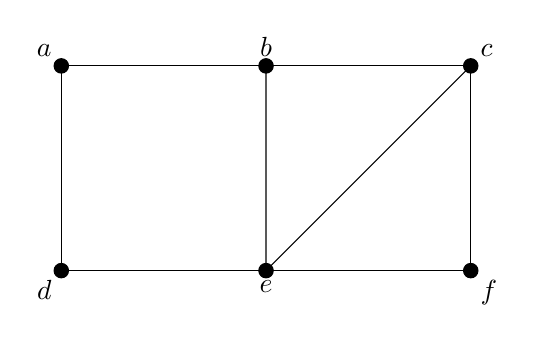
\begin{tikzpicture}[scale=1.3]
			\draw[fill=black] (0,0) circle (2pt) node[above left] {$a$};
			\draw[fill=black] (2,0) circle (2pt) node[above] {$b$};
			\draw[fill=black] (4,0) circle (2pt) node[above right] {$c$};
			\draw[fill=black] (0,-2) circle (2pt) node[below left] {$d$};
			\draw[fill=black] (2,-2) circle (2pt) node[below] {$e$};
			\draw[fill=black] (4,-2) circle (2pt) node[below right] {$f$};
			\draw (0,0) -- (4,0) --(4,-2) -- (0,-2) -- cycle;
			\draw (2,0) -- (2,-2) -- (4,0);
		\end{tikzpicture}
	\caption*{Figura 1.19: Grafo}
	\end{figure}
	\begin{enumerate}[label=\color{red}\alph*)]
		\item \db{Todos los caminos simples de $a$ a $f$.}
		
		Los caminos simples son aquellos que no repiten vértices. Los caminos simples de $a$ a $f$ son:
		\begin{itemize}[label=$-$]
			\item $a\to b\to c\to f$
			\item $a\to b\to e\to f$
		\end{itemize}
		\item \db{Todos los recorridos de $a$ a $f$.}
		
		Los recorridos incluyen todos los caminos posibles, sin restricciones de repetición de vértices. Los recorridos de $a$ a $f$ son:
		\begin{itemize}[label=$-$]
			\item $a\to b\to c\to f$
			\item $a\to b\to e\to f$
			\item $a\to b\to c\to e\to f$
			\item $a\to b\to e\to c\to f$
		\end{itemize}
		\item \db{La distancia de $a$ a $f$.}
		
		La distancia entre dos vértices es el número de aristas en el camino más corto entre ellos. 
		
		La distancia de $a$ a $f$ es 3, ya que el camino más corto es $a\to b\to e\to f$.
		\item \db{Todos los ciclos que incluyen al vértice $a$.}
		
		Los ciclos son caminos cerrados donde el único vértice que se repite es el inicial y final.
		
		Los ciclos que incluyen al vértice $a$ son:
		\begin{itemize}[label=$-$]
			\item $a\to b\to c\to f\to e\to d\to a$
			\item $a\to d\to e\to f\to c\to b\to a$
		\end{itemize}
		
		\item \db{El diámetro del grafo.}
		
		El diámetro de un grafo es la longitud del camino más largo entre dos vértices.
		
		El diámetro del grafo es 4, ya que el camino más largo es $a\to b\to c\to e\to f$
		\item \db{Todos los ciclos en $G$.}
		
	\end{enumerate}
	\item \lb{Considerar los multigrafos en la figura 1.20}
	
	
\begin{figure}[h]
	\centering
	\includegraphics{"Imágenes/Grafos 1.20.drawio"}
	\caption*{Figura 1.20: Grafos diversos}
\end{figure}
	
	\begin{enumerate}[label=\color{red}\alph*)]
		\item \db{¿Cuáles son conexos? Si un grafo no es conexo, encuentre sus componentes conexos}
		\item \db{¿Cuáles no tienen ciclos?}
		\item \db{¿Cuáles no tienen lazos?}
		\item \db{¿Cuáles son grafos simples?}
	\end{enumerate}
	
	\item \lb{Sea $G$ el grafo de la figura 1.21. Encontrar:}
	
	\begin{figure}[h]
		\centering
		\includegraphics{"Imágenes/Grafos 1.21.drawio"}
		\caption*{Figura 1.21: Grafo}
	\end{figure}
	\begin{enumerate}[label=\color{red}\alph*)]
		\item \db{Todos los caminos simples de $a$ a $c$}
		\item \db{Todos los ciclos}
		\item \db{El subgrafo $G'$ generado por $V'=\{b,c,d,e\}$}
		\item \db{El grafo $G-e$}
		\item \db{Todos los puntos de corte.}
		\item \db{Todos los puentes.}
	\end{enumerate}
	\item \lb{Dado  el grafo de la figura 1.22, determinar todos los subgrafos que resultan de eliminar un vértice. Demostrar que ninguno de los grafos obtenidos es isomorfo. ¿Tiene el grafo puntos de corte?}
	\begin{figure}[h]
		\centering
		\includegraphics{"Imágenes/Grafos 1.22.drawio"}
		\caption*{Figura 1.22: Grafo}
	\end{figure}
	
	\begin{figure}[h]
		\centering
		\includegraphics[width=\textwidth]{"Imágenes/Grafos 1.23.drawio"}
		\caption*{Figura 1.23: Grafos diversos}
	\end{figure}
	\item \lb{Determinar cuáles de los grafos de la figura 1.23 son Eulerianos.}
    
    Para que un grafo sea Euleriano, $\mathrm{def}(v)$ debe ser par $\forall v\in V$.
    
    El único grafo euleriano es $G_2$.
	\item \lb{Determinar cuáles de los grafos de la figura 1.23 son Hamiltonianos}
	\item \lb{Trazar todos los árboles que hay con exactamente seis vértices.}
	\item \lb{Encontrar todos los árboles generados del grafo de la figura 1.24.}
	
	\begin{figure}[h]
		\centering
		\includegraphics{"Imágenes/Grafos 1.24.drawio"}
		\caption*{Figura 1.24: Grafo}
	\end{figure}
	\item \lb{Encontrar el árbol generado de peso mínimo para el grafo de la figura 1.25.}
	
	\begin{figure}[h]
		\centering
		\includegraphics{"Imágenes/Grafos 1.24.drawio"}
		\caption*{Figura 1.25: Grafo ponderado}
	\end{figure}
	\item \lb{Sea $G=(V,E)$ un grafo con más de un vértice. Demostrar que las siguientes afirmaciones son equivalentes.}
	\begin{enumerate}[label=\color{red}\alph*)]
		\item \db{$G$ es un árbol.}
		\item \db{Cada par de vértices está unido por exactamente un camino simple.}
		\item \db{$G$ es conexo, pero $G\backslash\mathbf{e}$ es inconexo para cualquier arista $\mathbf{e}\in E$.}
		\item \db{$G$ no tiene ciclos, pero si a $G$ se agrega cualquier arista, entonces el grafo resultante tiene exactamente un ciclo.}
	\end{enumerate}
	\item \lb{Dibujar una representación plana, en caso de ser posible, de los grafos de la figura 1.26.}
	
	\begin{figure}[h]
		\centering
		\includegraphics[width=\textwidth]{"Imágenes/Grafos 1.26.drawio"}
		\caption*{Figura 1.26: Grafos diversos}
	\end{figure}
	
	\begin{figure}[h]
		\centering
		\includegraphics{"Imágenes/Grafos 1.27.drawio"}
		\caption*{Figura 1.27: Grafos diversos}
	\end{figure}
	\item \lb{Contar el número de vértices, aristas y regiones de cada mapa en la figura 1.27 y comprobar la fórmula de Euler. También, encontrar el grado de cada una de las regiones.}
	\item \lb{Encontrar el número mínimo de $n$ colores necesarios para pintar cada mapa en la figura.}
	\item \lb{Demostrar que un grafo plano $G$ es 5-coloreable, o se puede colorear con 5 colores.}
	\item \lb{Encontrar la matriz de adyacencia de los grafos de la figura 1.27.}
	\item \lb{Dibujar el grafo que tiene las siguientes matrices de adyacencia}
	\begin{enumerate}[label=\color{red}\alph*)]
		\item $\db{A=\begin{pmatrix}
				0 & 1 & 0 & 1 \\
				1 & 0 & 1 & 0 \\
				0 & 1 & 0 & 1 \\
				1 & 0 & 1 & 0
		\end{pmatrix}}$\qquad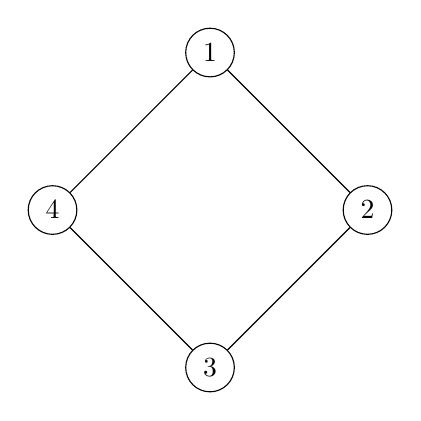
\begin{tikzpicture}[every node/.style={draw, circle}, scale=2, baseline=(current bounding box.center)]
		\node (1) at (0,0) {1}; 
		\node (2) at (1,-1) {2};
		\node (3) at (0,-2) {3};
		\node (4) at (-1,-1) {4};
		\draw (1) -- (2) -- (3) -- (4) -- (1);
	\end{tikzpicture}
	\item $\db{A=\begin{pmatrix}
			0 & 1 & 1 & 1 & 1 \\
			1 & 0 & 1 & 0 & 1 \\
			1 & 1 & 0 & 1 & 0 \\
			1 & 0 & 1 & 0 & 0 \\
			1 & 1 & 0 & 0 & 0
	\end{pmatrix}}$

\includegraphics{"Imágenes/16b.drawio"}
\item $\db{\begin{pmatrix}
		0 & 0 & 1 & 1 & 0 \\
		0 & 0 & 1 & 0 & 1 \\
		1 & 1 & 0 & 1 & 0 \\
		1 & 0 & 1 & 0 & 0 \\
		0 & 1 & 0 & 0 & 0
\end{pmatrix}}$

\includegraphics{"Imágenes/16c.drawio"}
	\end{enumerate}
	\begin{figure}[h]
		\centering
		\includegraphics{"Imágenes/Grafos 1.28.drawio"}
		\caption*{Figura 1.28: Grafo ponderado}
	\end{figure}
	\item \lb{Encontrar los árboles generadores de peso mínimo del grafo de la figura 1.28.}
	\item \lb{Encontrar el camino de peso mínimo entre los vértices $a$ y $f$ del grafo de la figura 1.28.}
	\item \lb{Sea $G=(V,E)$ un grafo. Definimos una relación $R$ dada por, dados $u,v\in V$ \[ u\sim v \]si y sólo si existe un camino desde $u$ hasta $v$. Demostrar que $R$ es una relación de equivalencia y explicar qué representa cada clase de equivalencia en esta relación.}
	\item \lb{Dado el grafo bipartito $K_{n,m}$ responder a las siguientes cuestiones:}
	\begin{enumerate}[label=\color{red}\alph*)]
		\item \db{Si $K_{n,m}$ contiene 16 aristas y $m\le n$, determinar  $m$ y $n$ tales que $K_{n,m}$ posea un camino cerrado euleriano pero no un ciclo hamiltoniano.}
		\item \db{Si $K_{n,m}$ contiene 16 aristas y $m\le n$, determinar  $m$ y $n$ tales que $K_{n,m}$ posea un camino cerrado euleriano y un ciclo hamiltoniano.}
		\item \db{¿Existe un ciclo hamiltoniano en $K_{4,4}$? ¿Y en $K_{4,5}$? ¿Y en $K_{4,6}$?}
		\item \db{Establecer una condición necesaria y suficiente para que $K_{n,m}$ sea hamiltoniano.}
	\end{enumerate}
	\item \lb{Un grafo $G$ no contiene ciclos y además tiene 526 vértices y 520 aristas. Si cada componente conexa de $G$ es un árbol, ¿cuántas componentes conexas forman $G$?}
	\item \lb{Si un árbol $G$ solo tiene vértices de grado 4 o de grado 1, probar que entonces el número de vértices de grado 1 que hay coincide con el doble de vértices de grado 4 más 2.}
	\item \lb{Construye un grafo plano con 10 aristas y 7 regiones distintas. Si no se puede, explica por qué.}
\end{enumerate}
\newpage
\section{Aritmética modular}
\begin{enumerate}[label=\color{red}\textbf{\arabic*)}, leftmargin=*]
	\item \lb{Calcular $\gcd(215,36)$ y $\gcd(334,562)$. Encontrar el mínimo común múltiplo de ambos pares de números y los $x_0$ e $y_0$ del Teorema de Bezout.}
	\begin{itemize}[label=\color{lightblue}$-$]
		\item $(215,36)$
		
		$\begin{array}{crcl}
			\gcd(215,36) & 215&=&36\cdot5+35\\
			\gcd(36,35) & 36 &=&35\cdot 1+1\\
			\gcd(35,1) & 35 &=&1\cdot35+0
		\end{array}$
		
		$\gcd(215,36) = 1$
		
		$\lcm(215,36)=\dfrac{|215\cdot36|}{\gcd(215,36)}=\dfrac{7740}{1}=7740$
		
		Para encontrar $x_0$ e $y_0$ en el Teorema de Bezout se usa el algoritmo extendido de Euclides $\left(\gcd(a,b)=ax+by\right)$.
		
		$\begin{aligned}
			1&=36-35\cdot1\\
			&=36-(215-36\cdot5)\\
			&=36-215+36\cdot5\\
			&=215\cdot(-1)+36\cdot6
		\end{aligned}$
		
		$1=215\cdot x_0+36\cdot y_0\longrightarrow\bboxed{\begin{array}{l}
			x_0=-1\\
			y_0=6
		\end{array}}$
		\item $(334,562)$
		
		$\begin{array}{crcl}
			\gcd(334,562) & 562 & = & 334\cdot1+228\\
			\gcd(334,228) & 334 & = & 228\cdot1+106\\
			\gcd(228,106) & 228 & = & 106\cdot2+16\\
			\gcd(106,16) & 106 & = & 16\cdot6+10\\
			\gcd(16,10) & 16 & = & 10\cdot1+6\\
			\gcd(10,6) & 10 & = & 6\cdot1+4\\
			\gcd(6,4) & 6 & = & 4\cdot1+2\\
			\gcd(4,2) & 4 & = & 2\cdot2+0
		\end{array}$
		
		$\gcd(334,562)=2$
		
		$\lcm(334,562)=\dfrac{|334\cdot562|}{\gcd(334,562)}=\dfrac{187708}{2}=96584$
		
		$\begin{aligned}
			2&=6-4\\
			&=6-(10-6)\\
			&=6\cdot2-10\\
			&=(16-10)\cdot2-10\\
			&=16\cdot2-10\cdot3\\
			&=16\cdot2-(10.6-16\cdot6)\cdot3\\
			&=16\cdot20-106\cdot3\\
			&=(228-106\cdot2)\cdot20-106\cdot3\\
			&=228\cdot20-106\cdot43\\
			&=228\cdot20-(334-228)\cdot43\\
			&=228\cdot63-334\cdot43\\
			&=(562-334)\cdot63-334\cdot43\\
			&=562\cdot63-334\cdot106
		\end{aligned}$
		
		$2=334\cdot x_0+562\cdot y_0\longrightarrow\bboxed{\begin{array}{l}
				x_0=-106\\
				y_0=63
		\end{array}}$
	\end{itemize}
	\item \lb{Demostrar que $\sqrt{2}$ no es un número racional.}
	
	$\sqrt{2}\in\Q$, por lo que $\sqrt{2}=\dfrac{p}{q}$ siendo $p,q\in\R$ y solo uno par para que pueda ser una fracción reducible $\left(\dfrac{2}{1},\dfrac{1}{2},\dfrac{3}{2},\dfrac{2}{3}\right)$.
	
	$\dfrac{p}{q}=\sqrt{2},\dfrac{p^2}{q^2}=2,p^2=2q^2$. Supongamos un cierto $m$, y si $m$ es par, su $m^2$ también $\left(\begin{array}{l}
		2\:\mathrm{par}\\
		2^2=4\:\mathrm{par}
	\end{array}\right)$
	
	Si $p^2=2q^2$, entonces $p$ es par por lo que entonces cierto $m$ es $p=2m,p^2=4m^2$, y como $p^2=2q^2,4m^2=2q^2$, que simplificado es $2m^2=q^2$ por lo que $q$ también es par, pero eso es contradictorio porque a lo sumo solo puede haber un numero par $\longrightarrow\sqrt{2}$ es irracional.
	\item \lb{Calcular $\gcd(18,256)$ y $\gcd(8316,10920)$. Encontrar el mínimo común múltiplo de ambos pares de números y los $x_0$ e $y_0$ del Teorema de Bezout.}
	
	\begin{itemize}[label=\color{lightblue}$-$]
		\item $(18,256)$
		
		$\begin{array}{crcl}
			\gcd(18,256) & 256 & = & 18\cdot14+4\\
			\gcd(18,4) & 18 & = & 4\cdot4+2\\
			\gcd(4,2) & 4 & = & 2\cdot2+0
		\end{array}$
		
		$\gcd(18,256)=2$
		
		$\lcm(18,256)=\dfrac{|18\cdot256|}{2}=\dfrac{4608}{2}=2304$
		
		$\begin{aligned}
			2 &=18-4\cdot4\\
			&=18-(256-18\cdot14)\cdot4\\
			&=18\cdot57-256\cdot4\\
		\end{aligned}$
		
		$2=18\cdot x_0+256\cdot y_0\longrightarrow\bboxed{\begin{array}{l}
				x_0=57\\
				y_0=-4
		\end{array}}$
	\item $(8316,10920)$
	
	$\begin{array}{crcl}
		\gcd(8316,10920) & 10920 & = & 8316\cdot1+2604\\
		\gcd(8316,2604) & 8316 & = & 2604\cdot3+504\\
		\gcd(2604,504) & 2604 & = & 504\cdot5+84\\
		\gcd(504,84) & 504 & = & 84 \cdot 6 +0
	\end{array}$
	
	$\gcd(8316,10920)=84$
	
	$\lcm(8316,10920)=\dfrac{|8316\cdot10920|}{84}=\dfrac{90810720}{84}=1081080$
	
	$\begin{aligned}
		84&=2604-504\cdot5\\
		&=2604-(8316-2604\cdot3)\cdot5\\
		&=2604\cdot16-8316\cdot5\\
		&=(10920-8316)\cdot16-8316\cdot5\\
		&=10920\cdot16-8316\cdot21
	\end{aligned}$
	
	$84=8316\cdot x_0+10920\cdot y_0\longrightarrow\bboxed{\begin{array}{l}
			x_0=-21\\
			y_0=16
	\end{array}}$
	\end{itemize}
	\item \lb{Enumerar todos los primos menores de 100.}
	
	$2,3,5,7,9,11,13,17,19,23,29,31,37,41,43,47,53,59,61,67,69,71,73,79,83,89,97$
	\item \lb{Sabiendo que $\gcd(a,b)=1$ probar las siguientes propiedades:}
	\begin{enumerate}[label=\color{red}\alph*)]
		\item $\db{\gcd(a+b,a-b)=1\text{ o }2}$
		\item $\db{\gcd(2a+b,2a+b)=1}$
	\end{enumerate}
	$\begin{array}{ccc}
		a+b=a-b & &a+2b=a\\
		\begin{array}{l}
			a+b=d\cdot m_1\\
			a-b=d\cdot m_2\\ \hline
			2a=d(m_1+m_2)
		\end{array} & \mathrm{o} & \begin{array}{l}
		\\
		\\ \hline
		2b=d(m_1-m_2)
		\end{array}
	\end{array}$
	
	En el caso de que $b$ o $a$ sean múltiplos de 2, puede ser que $\gcd(2a,2b)=\gcd(a,b)\cdot2=2$. En otro caso, $\gcd(a,b)=1$.
	\item \lb{Si $\gcd(a,b)=2$, obtener $\gcd(a-b,a^2-b^2)$.}
	
	\item \lb{Sea $d=\gcd(a,b)$. Demostrar que $\dfrac{a}{d}$ y $\dfrac{b}{d}$ son coprimos.}
	
	$d=ax+by$. Si $\dfrac{a}{d}$ y $\dfrac{b}{d}$ son coprimos $\longrightarrow\dfrac{d}{d}=\dfrac{a}{d}x+\dfrac{b}{d}y\longrightarrow1=\dfrac{a}{d}x+\dfrac{b}{d}y$
	
	$\gcd(a,b)=d=1$
	\item \lb{Realizar las siguientes operaciones y devolver el resultado en base 8 \[ 234_5+31_4\cdot21_3 \]}
	
	$\begin{array}{l}
		234)_5 = 2\cdot5^2+3\cdot5^1+4\cdot5^0=50+15+4=69)_{10}\\
		31)_{4}=3\cdot4^{1}+1\cdot4^{0}=12+1=13)_{10}\\
		21)_{3}=2\cdot3^1+1\cdot3^0=6+1=7)_{10}\\
		
		69+13\cdot7=160)_{10}=240)_{8}\\
	\end{array}$
	\item \lb{Encontrar un número entre 0 y 10000 que verifique todas las siguientes propiedades:}
	\begin{enumerate}[label=\color{red}\alph*)]
		\item \db{Las dos últimas cifras al escribirlo en base 8 son 03.}
		\item \db{Su última cifra en base 9 es 4.}
		\item \db{Es múltiplo de 7.}
	\end{enumerate}
	\item \lb{Realizar las siguientes operaciones en $\Z_{12}$ \[ 234+128\cdot54-(123+48\cdot7) \]}
	$\begin{array}{l}
		234\mod12=6\\
		128\cdot54=6912\mod12=0\\
		123\mod12=3\\
		48\cdot7=336\mod12=0\\
		6+0-3=3)_{12}
	\end{array}$
	\item \lb{Establecer cuáles de las siguientes congruencias son verdaderas.}
	\begin{enumerate}[label=\color{red}\alph*)]
		\item $\db{446\equiv278(\mod 7)}\quad\lb{\checkmark}$
		
		$\begin{array}{l}
			446\mod7=5\\
			278\mod7=5
		\end{array}$
		\item $\db{269\equiv413(\mod 12)}\quad\lb{\checkmark}$
		
		$\begin{array}{l}
			269\mod12=5\\
			413\mod12=5
		\end{array}$
		\item $\db{445\cancel{\equiv}536(\mod 18)}$
		
		$\begin{array}{l}
			445\mod18=13\\
			536\mod18=14
		\end{array}$
		\item $\db{793\cancel{\equiv}682(\mod 9)}$
		
		$\begin{array}{l}
			793\mod9=1\\
			682\mod9=7
		\end{array}$
		\item $\db{473\equiv369(\mod 26)}\quad\lb{\checkmark}$
		
		$\begin{array}{l}
			473\mod26=5\\
			369\mod26=5
		\end{array}$
		\item $\db{383\cancel{\equiv}126(\mod 15)}$
		
		$\begin{array}{l}
			383\mod 15=8\\
			126\mod 15=6
		\end{array}$
	\end{enumerate}
	\item \lb{Encontrar todos los números comprendidos entre -50 y 50 congruentes con 12 módulo de 21.}
	\item \lb{Encontrar $\varphi(37),\varphi(137),\varphi(275),\varphi(700)$ y $\varphi(201)$.}
	\begin{itemize}[label=\color{lightblue}$-$]
		\item $\varphi(37)=36$
		\item $\varphi(137)=136$
		\item $\varphi(275)=\varphi(5^2\cdot11)=(5^2-5)\cdot\varphi(11)=20\cdot10=200$
		\item $\varphi(700)=\varphi(2^2\cdot5^2\cdot7)=(2^2-2)\cdot(5^2-5)\cdot\varphi(7)=2\cdot20\cdot6=240$
		\item $\varphi(201)=\varphi(3\cdot67)=\varphi(3)\cdot\varphi(67)=2\cdot66=132$
	\end{itemize}
	
	\item \lb{Escribir las tablas de suma y multiplicación de $\Z_6$ y $\Z_7$.}
	
	$\begin{array}{|c|c|c|c|c|c|c|}
		\hline
		+ & 0 & 1 & 2 & 3 & 4 & 5 \\ \hline
		0 & 0 & 1 & 2 & 3 & 4 & 5 \\ \hline
		1 & 1 & 2 & 3 & 4 & 5 & 0 \\ \hline
		2 & 2 & 3 & 4 & 5 & 0 & 1 \\ \hline
		3 & 3 & 4 & 5 & 0 & 1 & 2 \\ \hline
		4 & 4 & 5 & 0 & 1 & 2 & 3 \\ \hline
		5 & 5 & 0 & 1 & 2 & 3 & 4 \\ \hline
	\end{array}\qquad\begin{array}{|c|c|c|c|c|c|c|}
	\hline
	\times & 0 & 1 & 2 & 3 & 4 & 5 \\ \hline
	0 & 0 & 0 & 0 & 0 & 0 & 0 \\ \hline
	1 & 0 & 1 & 2 & 3 & 4 & 5 \\ \hline
	2 & 0 & 2 & 4 & 0 & 2 & 4 \\ \hline
	3 & 0 & 3 & 0 & 3 & 0 & 3 \\ \hline
	4 & 0 & 4 & 2 & 0 & 4 & 2 \\ \hline
	5 & 0 & 5 & 4 & 3 & 2 & 1 \\ \hline
	\end{array}$
	
	$\begin{array}{|c|c|c|c|c|c|c|c|}
		\hline
		+ & 0 & 1 & 2 & 3 & 4 & 5 & 6 \\ \hline
		0 & 0 & 1 & 2 & 3 & 4 & 5 & 6 \\ \hline
		1 & 1 & 2 & 3 & 4 & 5 & 6 & 0 \\ \hline
		2 & 2 & 3 & 4 & 5 & 6 & 0 & 1 \\ \hline
		3 & 3 & 4 & 5 & 6 & 0 & 1 & 2 \\ \hline
		4 & 4 & 5 & 6 & 0 & 1 & 2 & 3 \\ \hline
		5 & 5 & 6 & 0 & 1 & 2 & 3 & 4 \\ \hline
		6 & 6 & 0 & 1 & 2 & 3 & 4 & 5 \\ \hline
	\end{array}\qquad\begin{array}{|c|c|c|c|c|c|c|c|}
	\hline
	\times & 0 & 1 & 2 & 3 & 4 & 5 & 6 \\ \hline
	0 & 0 & 0 & 0 & 0 & 0 & 0 & 0 \\ \hline
	1 & 0 & 1 & 2 & 3 & 4 & 5 & 6 \\ \hline
	2 & 0 & 2 & 4 & 6 & 1 & 3 & 5 \\ \hline
	3 & 0 & 3 & 6 & 2 & 5 & 1 & 4 \\ \hline
	4 & 0 & 4 & 1 & 5 & 2 & 6 & 3 \\ \hline
	5 & 0 & 5 & 3 & 1 & 6 & 4 & 2 \\ \hline
	6 & 0 & 6 & 5 & 4 & 3 & 2 & 1\\ \hline
	\end{array}$
	\item \lb{Encontrar usando el teorema de Bezout los inversos siguientes, en caso de que sea posible.}
	\begin{enumerate}[label=\color{red}\alph*)]
		\item \db{$12^{-1}$ en $\Z_5$}
		
		$12x\equiv1(\mod5)\longrightarrow x\equiv12^{-1}\mod(5)=12^{\varphi(5)-1}(\mod 5)=12^{3}(\mod5)=3(\mod5)\longrightarrow x=3$ en $\Z_5$
		\item \db{$20^{-1}$ en $\Z_{14}$}
		
		$\begin{array}{l}
			20x\equiv1(\mod14)\longrightarrow x\equiv20^{-1}(\mod14)=20^{\varphi(14)-1}(\mod14)=20^5(\mod14)=6\\
			\varphi(14)=\varphi(2)\cdot\varphi(7)=6
		\end{array}$
		
		$x=6$ en $\Z_{14}$
		\item \db{$(-21)^{-1}$ en $\Z_{13}$}
		
		$(-21)x\equiv1(\mod13)\longrightarrow x\equiv(-21)^{-1}(\mod13)=(-21)^{\varphi(13)-1}(\mod13)=(-21)^{11}(\mod13)=$
	\end{enumerate}
	\item \lb{Encontrar $a^{-1}$ en $\Z_m$ donde:}
	\begin{enumerate}[label=\color{red}\alph*)]
		\item \db{$a=37$ y $m=249$}
        
        $37^{-1}$ en $\Z_{249}\longrightarrow\gcd(37,249)=1$ Tiene inversa
        
        $\left(\begin{array}{c|cc}
        37 & 1 & 0 \\
        249 & 0 & 1
        \end{array}\right)\xrightarrow{F_2-6F_1}\left(\begin{array}{c|cc}
        37 & 1 & 0\\
        27 & -6 & 1
        \end{array}\right)\xrightarrow{F_1\longleftrightarrow F_2}\left(\begin{array}{c|cc}
        27 & -6 & 1\\
        37 & 1 & 0
        \end{array}\right)\xrightarrow{F_2-F_1}\left(\begin{array}{c|cc}
        27 & -6 & 1\\
        10 & 7 &-1
        \end{array}\right)\xrightarrow{F_1\longleftrightarrow F_2}\left(\begin{array}{c|cc}
        10 & 7 &-1\\
        27 & -6 & 1
        \end{array}\right)\xrightarrow{F_2-2F_1}\left(\begin{array}{c|cc}
        10 & 7 & -1\\
        7 & -20 & 3
        \end{array}\right)\xrightarrow{F_1\longleftrightarrow F_2}\left(\begin{array}{c|cc}
        7 & -20 & 3\\
        10 & 7 & -1
        \end{array}\right)\xrightarrow{F_2-F_1}\left(\begin{array}{c|cc}
        7 & -20 & 3\\
        3 & 27 & -4
        \end{array}\right)\linebreak\xrightarrow{F_1\longleftrightarrow F_2}\left(\begin{array}{c|cc}
        3 & 27 & -4\\
        7 & -20 & 3
        \end{array}\right)\xrightarrow{F_2-2F_1}\left(\begin{array}{c|cc}
        3 & 27 & -4\\
        1 & -74 & 11
        \end{array}\right)$
        
        $1=37\cdot(-74)+249\cdot11$
        
        $37^{-1}=-74\equiv175(\mod249)$
		\item \db{$a=15$ y $m=234$}
        
        $\gcd(15,234)=3\neq1$ No tiene inverso
	\end{enumerate}
	\item \lb{Resolver si es posible las siguientes ecuaciones en $\Z_5$.}
	\begin{enumerate}[label=\color{red}\alph*)]
		\item $\db{3x^2-7x+1=0}$
        
        $x=\dfrac{7\pm\sqrt{(-7)^2-4\cdot3\cdot1}}{2\cdot3}=\dfrac{7\pm\sqrt{49-12}}{den}$
		\item $\db{x^2+5x=1}$
	\end{enumerate}
	
	\item \lb{Resolver en $\Z_7$ el siguiente sistema de ecuaciones \[ \begin{cases}
			2x+3y=1,\\
			3x-2y=2.
		\end{cases} \]}
	\item \lb{Resolver la ecuación lineal de congruencia:}
	\begin{enumerate}[label=\color{red}\alph*)]
		\item $\db{3x\equiv2(\mod 8)}$
		
		$\begin{array}{l}
			x\equiv3^{-1}\cdot2(\mod8)=3^{\varphi(8)-1}\cdot2(\mod8)=3^3\cdot2(\mod8)=6(\mod8)\longrightarrow x=6\\
			\varphi(8)=\varphi(2^3)=2^3-2^2=4
		\end{array}$
		
		\item $\db{6x\equiv 5(\mod 9)}$
		
		$\begin{array}{l}
			x\equiv6^{-1}\cdot5(\mod9)=6^{\varphi(9)-1}\cdot5(\mod9)=6^5\cdot5(\mod9)=0(\mod9)\longrightarrow x=0\\
			\varphi(9)=\varphi(3^2)=3^2-3=6
		\end{array}$
		\item $\db{4x\equiv6(\mod 10)}$
		
		$\begin{array}{l}
			x\equiv4^{-1}\cdot6(\mod10)=4^{\varphi(10)-1}\cdot6(\mod10)=4^3\cdot6(\mod10)=4(\mod10)\longrightarrow x=4\\
			\varphi(10)=\varphi(2)\cdot\varphi(5)=4
		\end{array}$
	\end{enumerate}
	\item \lb{Encontrar el menor entero positivo $x$ tal que cuando $x$ se divide entre 3 se obtiene un resto igual a 2, cuando $x$ se divide entre 7 se obtiene un resto igual a 4 y cuando $x$ se divide entre 10 se obtiene un resto igual a 6.}
    
        $\begin{cases}
        x\equiv2(\mod3)\\
        x\equiv4(\mod7)\\
        x\equiv6(\mod10)
        \end{cases}\longrightarrow\begin{cases}
        70x\equiv1(\mod3)\\
        30x\equiv1(\mod7)\\
        21x\equiv1(\mod10)
        \end{cases}\longrightarrow\begin{array}{l}
        s_1=70^{\varphi(3)-1}(\mod3)=1\\
        s_2=30^{\varphi(7)-1}(\mod 7)=4\\
        s_3=21^{\varphi(10)-1}(\mod10)=1
        \end{array}$
        
        $x_0=2\cdot70\cdot1+4\cdot30\cdot4+6\cdot21\cdot1=746\equiv116(\mod210)$
	\item \lb{Encontrar soluciones enteras de las siguientes ecuaciones, cuando sea posible.}
	\begin{enumerate}[label=\color{red}\alph*)]
		\item $\db{5x+7y=4}$
        
        $5x\equiv4(\mod7)\longrightarrow x\equiv5^{\varphi(7)-1}\cdot4\longrightarrow x\equiv5(\mod7)$
		\item $\db{6x+24y=21}$
        
        $\begin{array}{l}
        6x\equiv21(\mod24)\longrightarrow x\equiv6^{\varphi(24)-1}\cdot21(\mod24)\longrightarrow x\equiv 0(\mod24)\\
        \varphi(24)=\varphi(2^3\cdot3)=\varphi(2^3)\cdot\varphi(3)=(2^3-2^2)\cdot\varphi(3)=4\cdot2=8
        \end{array}$
		\item $\db{14x+21y=49}$
        
        $14x\equiv49(\mod21)\longrightarrow14x\equiv7(\mod21)=\left\{14x\equiv\cancel{21x}-7x(\mod21)\right\}=-7x\equiv7(\mod21)\longrightarrow7x\equiv-7(\mod21)\longrightarrow7x\equiv14(\mod21)$
        
        $\begin{array}{l}
        x\equiv7^{\varphi(21)-1}\cdot14(\mod21)\longrightarrow x\equiv0(\mod21)\\
        \varphi(21)=\varphi(3)\cdot\varphi(7)=12
        \end{array}$
        
	\end{enumerate}
	\item \lb{Encontrar los inversos siguientes a partir de la función $\varphi$ de Euler:}
	\begin{enumerate}[label=\color{red}\alph*)]
		\item \db{$20^{-1}$ en $\Z_9$}
        
        $20^{\varphi(9)-1}(\mod 9)=20^5(\mod 9)=5(\mod 9)$
        
        $\varphi(9)=\varphi(3^2)=3^2-3=6$
		\item \db{$7^{-1}$ en $\Z_{12}$}
        
        $7^{\varphi(12)-1}(\mod12)=7^3(\mod12)=7$
        
        $\varphi(12)=\varphi(2^2)\cdot\varphi(3)=(2^2-2)\cdot\varphi(3)=4$
	\end{enumerate}
	\item \lb{Resolver el siguiente sistema:\[ \begin{cases}
			2x\equiv3(\mod 7)\\
			x\equiv 1(\mod9)\\
			x\equiv3(\mod 8)\\
			x\equiv0(\mod11)
		\end{cases} \]}
	
    $\begin{cases}
    			x\equiv5(\mod 7)\\
    			x\equiv 1(\mod9)\\
    			x\equiv3(\mod 8)\\
    			x\equiv0(\mod11)
    		\end{cases}\longrightarrow\begin{cases}
            			792x\equiv1(\mod 7)\\
            			616x\equiv 1(\mod9)\\
            			693x\equiv1(\mod 8)\\
            			504x\equiv1(\mod11)
            		\end{cases}\longrightarrow\begin{cases}
                    			x\equiv1(\mod 7)\\
                    			4x\equiv 1(\mod9)\\
                    			5x\equiv1(\mod 8)\\
                    			9x\equiv1(\mod11)
                    		\end{cases}\longrightarrow\begin{array}{l}
                            s_1=1^{\varphi(7)-1}(\mod 7)=1\\
                            s_2=4^{\varphi(9)-1}(\mod 9)=7\\
                            s_3=5^{\varphi(8)-1}(\mod8)=5\\
                            s_4=9^{\varphi(11)-1}(\mod11)=5
                            \end{array}
                    	$
                        
    $x_0=5\cdot792\cdot1+1\cdot616\cdot7+3\cdot693\cdot5+\cancel{0\cdot504\cdot5}=18667\equiv2035(\mod5544)$
   	\item \lb{Probar que si son ciertas las siguientes propiedades, y si no lo son, dar un ejemplo que muestre que son falsas.}
	\begin{enumerate}[label=\color{red}\alph*)]
		\item \db{Si $a|b,a|c,a|d$, entonces $a|b\cdot p+c\cdot q+d\cdot r$, donde $a,b,c,d,p,q,r\in\Z$.}
		\item \db{Si $a|b,a|c\cdot d$ entonces $a|b\cdot k`c\cdot l$, donde $a,b,c,d,k,l\in\Z$.}
	\end{enumerate}
	\item \lb{Resuelve las siguientes ecuaciones en congruencias:}
	\begin{enumerate}[label=\color{red}\alph*)]
		\item \db{$28x+13=0$ en $\Z_{45}$}
		
		$28x\equiv-13(\mod45)\longrightarrow28x\equiv32(\mod45)\longrightarrow x\equiv28^{-1}\cdot32(\mod45)$
		\item \db{$51x+32=0$ en $\Z_{60}$}
		\item \db{$36x+44y=28, x,y\in \Z$}
		\item \db{$x\equiv7(\mod9)$}
		
		$x=7$
		\item \db{$x\equiv13(\mod12)$}
		
		$x=1$
	\end{enumerate}
	\item \lb{Cada vez que Pablo va a la tiendo se compra tres camisetas, mientras que cada vez que Antonio visita la tienda se compra seis. ¿Es posible que se hayan acabado comprando un total de 152 camisetas? ¿Y 153? En los casos en los que sea posible, ¿cuántas visitas hizo cada uno a la tienda?}
	\item \lb{Una empresa fabrica dos modelos de coche. Para el primero, requiere 24 tornillos, mientras que para el segundo requiere 26.}
	\begin{enumerate}[label=\color{red}\alph*)]
		\item \db{Si el uno de mayo se requirieron 224 tornillos, ¿cuántos coches se hicieron de cada modelo?}
		\item \db{Si el primer modelo se vende por 10000 euros, mientras que el segundo se vende por 12000 euros, ¿cuántos modelos debería vender la empresa para obtener el máximo beneficio?}
	\end{enumerate}
\end{enumerate}
\newpage
\section{Combinatoria}
\begin{enumerate}[label=\color{red}\textbf{\arabic*)}, leftmargin=*]
	\item \lb{Calcular $\dfrac{7!}{10!}$ y $\dfrac{12!}{10!}$}
    \begin{itemize}[label=$-$]
    \item $\dfrac{7!}{10!}=\dfrac{1}{720}$
    \item $\dfrac{12!}{10!}=132$
    \end{itemize}
    \item \lb{Simplificar $\dfrac{n!}{(n-1)!}$ y $\dfrac{(n+2)!}{n!}$}
    \begin{itemize}[label=$-$]
    \item $\dfrac{n!}{(n-1)!}=\dfrac{\cancel{n!}}{(n-1)\cdot\cancel{n!}}=\dfrac{1}{(n-1)}$
    \item $\dfrac{(n-2)!}{n!}=\dfrac{\cancel{n!}\cdot(n+1)\cdot(n+2)}{\cancel{n!}}=(n+1)\cdot(n+2)=n^2+3n+2$
    \end{itemize}
    \item \lb{Supongamos que tenemos 5 libros de historia, 3 de sociología, 6 de antropología y 4 de psicología. Encontrar el número $n$ de posibilidades entre las que un estudiante puede escoger:}
    \begin{enumerate}[label=\color{red}\alph*)]
    	\item \db{Uno de los libros.}
        
        $n_a=5+3+6+4=18$ casos posibles.
        \item \db{Un libro de cada tema.}
        
        $n_b=5\cdot3\cdot6\cdot4=360$ casos posibles.
    \end{enumerate}
    \item \lb{En un curso de historia hay 8 estudiantes hombres, 6 estudiantes mujeres y 2 no binarios. Encontrar los posibles casos de elegir:}
    \begin{enumerate}[label=\color{red}\alph*)]
    	\item \db{Un representante del curso.}
        
        $n_a=8+6+2=16$ casos posibles.
        \item \db{Dos representantes del curso: un hombre y una mujer.}
        
        $n_b=8\cdot6=48$ casos posibles.
        \item \db{Dos representantes del curso: una mujer y un no binario.}
        
        $n_c=6\cdot2=12$ casos posibles.
        \item \db{Un presidente y un vicepresidente.}
        
        $n_d=$ total de estudiantes $\cdot$ (total de estudiantes $- 1$) $=(8+6+2)\cdot(8+6+2-1)=16\cdot15=240$ casos posibles
    \end{enumerate}
    \item \lb{Entre $A$ y $B$ hay cuatro líneas de autobuses, y entre $B$ y $C$ hay tres líneas de autobuses. Encontrar el número de formas en que una persona puede viajar en autobús:}
    \begin{enumerate}[label=\color{red}\alph*)]
        \item \db{De $A$ a $C$ pasando por $B$.}
        
        $n_a=4\cdot3=12$ posibles
        \item \db{En viaje de ida y vuelta de $A$ a $C$ pasando por $B$.}
        
        $n_b=12\cdot12=144$ formas posibles
        \item \db{En viaje de ida y vuelta de $A$ a $C$ pasando por $B$ pero sin usar una línea de autobús más de una vez.}
        
        $n_c=4\cdot 3\cdot(4-1)=36$ formas posibles
    \end{enumerate}
    \item \lb{Encontrar todas las posibles de permutaciones distintas que pueden formarse con todas las letras de las palabras PATOS, PARADAS y SOCIOLÓGICAS.}
    \begin{itemize}[label=$-$]
    \item PATOS $\longrightarrow n=5\longrightarrow P(n)=n!\longrightarrow P(5)=5!=120$ formas posibles.
    \item PARADAS $\longrightarrow n=7\longrightarrow P(7)=7!=5\,040$ formas posibles.
    \item SOCIOLÓGICAS $\longrightarrow n=12\longrightarrow P(12)=12!=479\,001\,600$ formas posibles.
    \end{itemize}
    
    \item \lb{En un curso hay 16 hombre, 14 mujeres y 3 no binarios. Encuentre el número de maneras de elegir:}
    \begin{enumerate}[label=\color{red}\alph*)]
    	\item \db{Un comité de 4 miembros.}
        
        $C_a(16+14+3,\,4)=C_a(33,4)=\dbinom{33}{4}=\dfrac{33!}{4!\cdot(33-4)!}=40\,920$ formas posibles de elegir un comité de 4 personas.
        \item \db{Un comité de 6 miembros con 2 hombres, mujeres y 2 no binarios.}
        
        $C_b=C_b(16,2) \cdot C(14,2)\cdot C(3,2)=\dbinom{16}{2}\cdot\dbinom{14}{2}\cdot\dbinom{3}{2}=\dfrac{16}{2!\cdot(16-2)!}\cdot\dfrac{14!}{2!\cdot(14-2)!}\cdot\dfrac{3!}{2!\cdot(3-2)!}=120\cdot91\cdot3=32\,760$
        \item \db{Un presidente, un vicepresidente y un tesorero.}
        
        $n_c=n\cdot(n-1)\cdot(n-2)=33\cdot32\cdot31=32\,736$ formas de elegir un presidente, un vicepresidente y un tesorero.
    \end{enumerate}
    \item \lb{Una caja contiene 8 calcetines azules y 6 calcetines rojos. Encontrar el número de formas en que es posible extraer dos calcetines de la caja si:}
    \begin{enumerate}[label=\color{red}\alph*)]
    	\item \db{Pueden ser de cualquier color.}
        
        $n_a=8\cdot6=48$ formas posibles.
        \item \db{Deben ser  del mismo color.}
        
        $n_b=\dbinom{8}{2}+\dbinom{6}{2}=\dfrac{8!}{2!\cdot(8-2)!}+\dfrac{6!}{2!\cdot(6-2)!}=43$ formas posibles.
    \end{enumerate}
    \item \lb{Encontrar el número de comités de 5 miembros con un director que es posible escoger entre un grupo de 12 personas.}
    
    Seleccionamos una persona del grupo de 12 como director y luego seleccionamos 4 personas de las 11 restantes para completar el comitée:
    
    $\dbinom{12}{1}\cdot\dbinom{11}{4}=\dfrac{12!}{1!\cdot(12-1)!}\cdot\rbinom{11}{4}=$
    \item \lb{Encontrar el número mínimo de estudiantes necesario para garantizar que al menos cinco de ellos están en cada uno de los cursos de un grado de cuatro años.}
\end{enumerate}
\end{document}

